\documentclass[UTF8]{ctexart}

\usepackage{graphicx}
\graphicspath{{graphics/}}

\pagestyle{plain} %没有页眉,页脚包含一个居中的页码

\setcounter{tocdepth}{1} %%目录深度1
\usepackage[hidelinks]{hyperref} %%目录超链接

\usepackage{draftwatermark} %%水印
\SetWatermarkText{读书笔记}
\SetWatermarkScale{0.25}
\SetWatermarkLightness{0.9}

\title{\heiti \zihao{-2}读书笔记}
\author{刘继超}
\date{ }


\begin{document}
	
	\maketitle	
	\thispagestyle{empty}
	
	\renewcommand{\abstractname}{\zihao{3}{序言}}
	
	\begin{abstract}
		\zihao{-4}
	
		\centering{鉴于往事,好玩且有资于吹比}
	\end{abstract}

	\newpage
	
	\pagenumbering{Roman}
	
	\tableofcontents
	
	\newpage
	
	\pagenumbering{arabic}
	
	\setcounter{page}{1} 
	
	\section{赛博空间伦理学}
	
		\centering{哈姆林克}
	
		\begin{enumerate}
		
			\item 历史上出现的“技术文化”,使得技术发展的道德责任问题尤为紧迫。
			自从欧洲中世纪后期以来,商人资本家阶层出现了,他们表现出对控
			制自然、掌握社会的能力的强烈信心。这种情况是由对技术进步和人
			类完善性的几乎无节制的信仰激发的。这种扩张的情绪没有受到道德
			因素的制止。总有新的目标,也总有实现这些目标的新工具。技术雄心
			的道德性质没有受到过质疑,它们的前提从未经受过严肃的检验。在
			“技术文化”的发展过程中,人类把自己从自然力中解放了出来,与此
			同时,它使自己臣服于技术工具的威力。
		
			\item 对前瞻性评价的根本批评,针对着作为技术预测根基的各种假设。技
			术预测从一个归纳主义的基础出发,受到这一假定的指导,即人可以
			在过去有限数量的观察基础上对未来做出预言。在18 世纪,休谟反对
			这种归纳主义。他指出,没有逻辑的证据证明可以得出这样的结论:我
			们不知道的现象会与我们确实知道的现象相像。归纳主义必须假定历
			史过程具有内在连续性。它需要承认存在不可移易的历史命运的法则,
			物质科学可以对物理世界的规律性给出这样的法则,但是没有经验证
			据支持这一信念:类似的规律性在社会环境中也有效。当然,在人类
			社会历史中可以观察到一些趋势,但是它们与决定社会的运动从而提
			供关于社会未来的可靠预测的自然法则截然不同。
		
			\item 在为市场作辩护时,常常有人提及市场的竞争效果。但是,在这个论
			点中——有意或者无意——在“自由市场”概念和“开放竞争”概念
			之间存在一个误导性的混淆。在国际市场上,这两个概念是互相排斥
			的。市场越是自由,就越会出现集中,结果竞争就越少。非管制市场
			的思想假定存在着平等参与者之间的竞争。但是现实中总是存在实力
			或强或弱的参与者,他们之间的竞争产生出赢家和输家。全球市场上
			的竞争是残酷无情的竞争:一种军事的、侵略性的竞争变种,在其中
			竞争对手被驱逐出市场。这种形式的竞争导致集中程度不断增强。只
			有强有力的公共干预才能保证自由与平等的竞争关系。但是这种干预
			又限制了市场的自由。这是一个典型的进退两难的情形。甚至把自身
			利益看作是经济增长的主要动力并且相信这最终有利于集体利益的亚
			当·斯密,也看到完全不加控制的自身利益会危害合作,导致垄断。
	
			\item 对苏格拉底来说,对我们自己的假定进行批判的审查是所有严肃反思
			的核心。苏格拉底确信:我们的观念常常是更多地由信仰而非知识而
			决定,我们常常没能解释这些信仰。苏格拉底方法不忽视事实性知识
			的重要性,但是期望探索它的意义。苏格拉底是在寻找智慧,因此,他
			问我们是否知道我们的知识究竟代表什么。他的考察无情地揭示出我
			们常常谈论许多我们很少了解的东西,而且我们时常甚至不了解我们
			自己的想法。
			
		\end{enumerate}
	
	\newpage
	
	\section{机器之心}
	
		\centering{雷·库兹韦尔}
	
		\begin{enumerate}
			\item 尽管宇宙中的无序性在增加,但进化过程却可能让复杂度和有序度同
			时存在并且增加。进化是一个过程,不是封闭的系统,它受外部影响,
			同时又可以对其包含的无序性善加利用。进化过程的关键要求之一就
			是要将进化结果以“书面”方式记录下来,否则这一过程将注定一直
			在为已经解决的问题反复寻找答案。
			
			\item 如果一个科学家说某件事情是可能的,那他基本上不会出错。但如果
			他说,某件事情是不可能的,那他就极有可能出错。探索可能性极限
			的唯一方法就是再冒险一点,朝不可能的方向再迈进一步。所有先进
			的技术都与魔法无异。
			
				\rightline{——英国科幻小说家亚瑟·克拉克的“克拉克三定律”}
			
			\item	时间与混沌定律:在一段过程中,重大事件(即能够改变过程性质的
			事件或能够对过程的未来产生重大影响的事件)的间隔会随着混沌的程度加长
			或缩短。混沌指的是在某一过程中的相关事件中无序(随机事件)的数量。
			混沌增加定律:如果混沌以指数级速度增长,时间的流逝将以指数级速度放缓。
			随着时间流逝,发生重大事件的时间间隔会变长)。
			加速回报定律:秩序以指数级速度增加,时间也随之以指数级速度加速。
			进化过程中的加速回报定律:进化过程不是一个封闭系统,因此进化可以利用
			更大型系统中的混沌,并为自身的多样性汲取力量。进化建立在自身不断增强的
			有序性上,在进化过程中,有序性以指数级速度增加,因此,回报加速。
			有序就是与某个目的相匹配的信息。衡量秩序的等级,就是衡量信息与目的的匹配程度。
			
			\item 计算机一方面需要依靠其创造者的大脑设计结构,同时又被植入所创
			造物种的大脑和身体中,与之融为一体。创造物种的大脑和神经系统
			被分区块输送至计算机系统中,最终代替计算机中的信息处理部件。各
			种实际和伦理问题会阻碍但无法阻止这一过程的发生。根据加速回报
			定律,我们可以预测,发明技术的物种与其所创造的技术最终将完全
			融合在一起。在走到这一步之前,技术创造型物种及其所发明的技术
			可能会进行自我毁灭。进化过程的彻底毁灭是阻止加速回报定律指数
			增长的唯一方法。强大的技术自被创造初就有巨大的毁灭潜力,可以
			将技术创造型物种及其发明的技术共同生存的生态环境全部摧毁。
			
		\end{enumerate}
	
	\newpage
	
	\section{逃避自由}
	
		\centering{埃里希·弗洛姆}
	
		\begin{enumerate}
	
			\item 现代人摆脱了前个人状态社会纽带的束缚,但并未获得积极意义上的
			实现个人自我的自由,也就是说,他无法自由地表达自己的思想、情
			感及感官方面的潜力。自由虽然给他带来了独立与理性,但也使他孤
			立,并感到焦虑和无能为力。他无法忍受这种孤立,他面临着两种选
			择:或者逃避自由带来的重负,重新建立依赖和臣服关系;或者继续
			前进,力争全面实现以人的独一无二性及个性为基础的积极自由。
			
			\item 弗洛伊德接受了传统的人与社会基本对立冲突的观念及传统的性恶论。
			他认为人基本是反社会的。社会必须驯化他,必须允许他直接满足某
			些无法消除的生物冲动(drives)。但社会在绝大多数情况下必须净化
			并巧妙抑制人的基本冲动。在社会对人的自然冲动的压抑下,奇妙的
			事情发生了:被压抑的冲动变成具有文化价值的奋斗动力(strivings),
			而且成为文化的人文基础,弗洛伊德用“升华”来表示这种由压抑而
			成为文明行为的奇特转变。一般来说,人的基本冲动的满足与文化的
			关系是相反的;压抑越大,文化程度便越高(患神经症的危险也越大)。
			按照弗洛伊德的理论,个人与社会的关系基本固定不变:个人基本保
			持不变,只是在社会对他的自然冲动施加更大压力(升华也增强了)或
			允许其得到更大满足(因此牺牲了文化)时,才发生变化。
			
			\item 人的自由增长过程与个人的成长过程一样具有辩证特征。一方面,它
			是一个人的力量与完整性不断增强,对自然的支配越来越得心应手的
			过程,是理性能力以及与他人的联系日益紧密的过程;但另一方面,这
			个日益加剧的个体化进程又意味着孤独感和不安全感日益增强,也意
			味着个人对自己在宇宙中的地位,对生命的怀疑增大,个人的无能为
			力感和微不足道感也日益加深。
	
			\item 如果我们分析宗教或者政治学说的心理意义,就必须区分两个问题,我
			们必须研究新学说创立者的性格结构,并尽量弄清其人格中的什么特
			质促成了这方面的特殊思想。另一个问题是研究这种学说所吸引的社
			会群体的心理动机,而不是学说创立者的动机。任何一种学说或思想
			的影响取决于它所吸引的那些人性格结构中的心理需求程度大小。要
			是该思想答复了某些社会群体强大的心理需求,它将成为历史上的一
			种强大力量。当然,这两个问题,即领袖的心理和信徒的心理,是密切
			相连的。
			
			\item 怀疑是现代哲学的起点。平息怀疑的需求是现代哲学及科学发展的最
			强大刺激。但是,虽然理性回答解决了许多理性怀疑,可非理性怀疑却
			没有消失,只要人还未从消极被动的自由进步到积极主动的自由,它
			便不可能消失。平息怀疑的现代企图,无论是强制性地奋斗以渴求成
			功,还是坚信有关事物的无限知识可以回答对肯定的渴望,抑或臣服
			于一个负有“肯定”责任的领袖,这些方案都只能消除对怀疑的主观
			意识。在人未克服自己的孤立,并从人的需求角度使自己在世界中的
			地位富有意义之前,怀疑本身是无法消失的。
			
			\item 社会进程通过决定个人的生活模式,即与他人以及劳动的关系,塑造
			了他的性格结构;新的宗教、哲学及政治等意识形态源于这个变化了
			的性格结构,却又诉诸它,并强化、满足、稳定了它;新形成的性格特
			质反过来又成为经济进一步发展的重要因素,影响社会的进程;虽然
			最初它们是作为对新经济力量之威胁的反作用发展起来的,但渐渐地
			它们又成为推动并强化新经济发展的生产力。
			
			\item 我们认为下面这些真理是不言而喻的:人人生而平等,造物者赋予他
			们若干不可剥夺的权利,其中包括生命权、自由权和追求幸福的权利。
			我们认为下面这些真理是不言而喻的:人人演化各有不同,出生就具
			有某些可变的特性,其中包括生命和追求快感。
			
			\item 我们发现有三种施虐倾向,它们或多或少地纠缠在一起。一是让别人
			依赖自己,以绝对无限的权力通知他们,以便让他们仅仅成为自己手
			中的工具;二是不但有以这种绝对方式统治别人的冲动,而且还要剥
			削、利用、偷窃、蚕食别人,把别人吸干榨净,不但包括物质,而且还
			包括情感与智慧之类的精神方面;第三种施虐倾向是希望别人受磨难,
			或看别人受磨难。其目的是主动伤害、羞辱他们,要看他们狼狈不堪
			的窘相。
			
			\item 惟有当我们有能力拥有自己的想法时,表达我们想法的权力才有价值;
			惟有当内在的心理状态能使我们可以确定自己的个人地位时,不受外
			在权威控制的自由,才能成为一项永恒的收获。
	
		\end{enumerate}
	
		\newpage
	
	
	\section{数学之美}
	
		\centering{吴军}
	
		\begin{enumerate}
		
			\item 最大熵原理指出,对一个随机事件的概率分布进行预测时,我们的预测
			应当满足全部已知的条件,而对未知的情况不要做任何主观假设。在
			这种情况下,概率分布最均匀,预测的风险最小,概率分布的信息熵
			最大。
		
		\end{enumerate}

	\newpage

	\section{毛泽东选集}
	
		\centering{毛泽东}
	
		\begin{enumerate}
		
			\item 在绝对的总的宇宙发展过程中,各个具体过程的发展都是相对的,因
		而在绝对真理的长河中,人们对于在各个一定发展阶段上的具体过程
		的认识只具有相对的真理性。无数相对的真理之总和,就是绝对的真
		理。
		
			\item 人的正确思想是从哪里来的?是从天上掉下来的吗?不是。是自己头脑 
	    里固有的吗?不是。人的正确思想,只能从社会实践中来,只能从社会的生产斗争、阶
	    级斗争和科学实验这三项实践中来。人们的社会存在,决定人们的思想。而代表先进阶
		级的正确思想,一旦被群众掌握,就会变成改造社会、改造世界的物质力量。人们在社
		会实践中从事各项斗争,有了丰富的经验,有成功的,有失败的。无数客观外界的现象
		通过人的眼、耳、鼻、舌、身这五个官能反映到自己的头脑中来,开始是感性认识。这
		种感性认识的材料积累多了,就会产生一个飞跃,变成了理性认识,这就是思想。这是
		一个认识过程。这是整个认识过程的第一个阶段,即由客观物质到主观精神的阶段,由
		存在到思想的阶段。这时候的精神、思想(包括理论、政策、计划、办法)是否正确地
		反映了客观外界的规律,还是没有证明的,还不能确定是否正确,然后又有认识过程的
		第二个阶段,即由精神到物质的阶段,由思想到存在的阶段,这就是把第一个阶段得到
		的认识放到社会实践中去,看这些理论、政策、计划、办法等等是否能得到预期的成功。
		一般的说来,成功了的就是正确的,失败了的就是错误的,特别是人类对自然界的斗争
		是如此。在社会斗争中,代表先进阶级的势力,有时候有些失败,并不是因为思想不正
		确,而是因为在斗争力量的对比上,先进势力这一方,暂时还不如反动势力那一方,
		所以暂时失败了,但是以后总有一天会要成功的。人们的认识经过实践的考验,又会产
		生一个飞跃。这次飞跃,比起前一次飞跃来,意义更加伟大。因为只有这一次飞跃,才
		能证明认识的第一次飞跃,即从客观外界的反映过程中得到的思想、理论、政策、计划、
		办法等等,究竟是正确的还是错误的,此外再无别的检验真理的办法。而无产阶级认识
		世界的目的,只是为了改造世界,此外再无别的目的。一个正确的认识,往往需要经过
		由物质到精神,由精神到物质,即由实践到认识,由认识到实践这样多次的反复,才能
		够完成。这就是马克思主义的认识论,就是辩证唯物论的认识
		
			\item 理性认识依赖于感性认识,感性认识有待于发展到理性认识,这就是
		辩证唯物论的认识论。马克思主义哲学认为十分重要的问题,不在于
		懂得了客观世界的规律性,因而能够解释世界,而在于拿这种对于客
		观规律性的认识去能动地改造世界。
		
		\end{enumerate}
	
	\newpage

	\section{乌合之众}

		\centering{古斯塔夫·勒庞}

		\begin{enumerate}
	
			\item 有意识人格的消失,无意识人格的得势,思想和情感因暗示和相互传
			染作用而转向一个共同的方向,以及立刻把暗示的观念转化为行动的
			倾向,是组成群体的个人所表现出来的主要特点。
	
			\item 刺激因素对群体和个人有控制作用,但是孤立的个人具有主宰自己的
			反应行为的能力,群体则缺乏这种能力。刺激群体的因素多种多样,群
			体总是屈从于这些刺激,因此群体也极为多变。
			
			\item 如果有人毁掉那些博物馆和图书馆,如果有人把教堂前石板路上那些
			在宗教鼓舞下建立起的一切作品和艺术纪念物统统推掉,人类伟大的梦想还会
			留下些什么呢?让人们怀抱着那些希望和幻想吧,不然他们
			是活不下去的。这就是存在着诸神、英雄和诗人的原因。科学承担起
			这一任务已经有五十年的时间,但是在渴望理想的心灵里,科学是有
			所欠缺的,因为它不敢做出过于慷慨的承诺,因为它不能撒谎。
			
		\end{enumerate}

	\newpage
	
	\section{苏菲的世界}
	
		\centering{乔斯坦·贾德}
	
		\begin{enumerate}
		
			\item 在柏拉图的理论中,现实世界最高层次的事物是那些我们用理性来思
			索的事物。但对亚里士多德而言,现实世界最高层次的事物是那些我
			们用感官觉察的事物。亚里士多德指出,我们对于自己的感官未曾经
			验过的事物就不可能有意识。柏拉图则会说,不先存在于理型世界中
			的事物就不可能出现在自然界中。亚里士多德认为,我们拥有的每一
			种思想与意识都是通过我们看到、听到的事物而进入我们的意识。不
			过我们也具有与生俱来的理性,因此天生就能组织所有的感官印象,并
			且将他们加以整理和分类,所以才会产生诸如“石头”、“植物”等概
			念。
		
			\item 生命本来就是悲伤而严肃的。我们来到这个美好的世界里,彼此相逢,
			彼此问候,并结伴同游一段短暂的时间。然后我们就失去了对方,并
			且莫名其妙就消失了,就像我们莫名其妙来到这世界上一样。
		
			\item 正如休谟说的,自我只不过是一束不同的知觉以无法想象的速度接连而来,不断改变并移动的过程。他说,心灵是一个剧场。在这个剧场里,不同的感官认知在各种位置和情况下轮流出现、经过、再现、消退和融合。我们心中有的只是这些来来去去的知觉和感觉,并没有一定的“自我同一性(personalidentity)”。
			
			\item 康德将“时间”和“空间”称为我们的两种“直观形式”(form of intuition)。他强调我们心灵中的这两种形式先于一切经验,我们在还没有经验事物之前,就可以知道我们感知到的将是一个发生在时间和空间里的现象。休谟认为我们无法证明因果律,康德则认为因果律的存在正是人类理性的特色。正因为人类的理性可以感知事物的因果,因此因果律是绝对且永恒不变的。康德认为“事物本身 das Ding an sich”和“我眼中的事物 das Ding fuer mich”是不一样的。我们永远无法确知事物“本来”的面貌。我们所知的只是我们眼中“看到”的事物。从另一个角度来看,我们在每一次经验之前都可以预知我们的心灵将如何认知事物。
			
			人类对世界的观念受到两种因素左右。一个是我们必须通过感官才能知道的外在情况,称之为知识的原料。另一个因素是人类内在的情况,例如我们所感知到的事物都是发生在时空之中,而且符合不变的因果律,称为知识的形式。
			
			作为一个由物质形成的存在者,我们完全属于自然界,因此受到因果律的支配,在这种情况下我们没有自由意志可言。可是作为一个有理性的存在者,我们在康德的“物自身”中占有一席之地。只要在我们追随我们的“实践理性”,并因此得以做道德上的抉择时,我们才有自由意志可言。因为当我们遵守道德法则时,我们也正是制定这项法则的人。
			
			康德死后葬在哥尼斯堡。他的墓碑上刻有一句他最常被人引用的名言:“有两件事物我越是思考越觉得神奇,心中也越充满敬畏,那就是我头顶上的星空和我内心的道德准则。他们向我印证:上帝在我头顶,也在我心中。”
			
			\item 黑格尔认为,思想(或理性)的历史就像一条河流。思考方式受到宛如河水般向前推进的传统思潮和当时的物质条件的影响。因此永远无法宣称任何一种思想永远是对的。只不过就所置身之处而言,这种思想可能是对的。
			
			黑格尔指出,每一种新思想通常都是以前人的旧思想为基础,而一旦有一种新思想被提出来,马上就会出现另一种和它抵触的思想,于是这两种对立的思想之间就会产生一种紧张状态,但这种紧张状态又会因为有人提出另一种融合了两种思想长处的思想而消除。
			
			黑格尔的“理性”有一种动态的逻辑。既然“事实”的特性就是会有相反的事物,因此要描述事实就必须同样描述与事实相反的事物。
			
			
			\item 祁克果和康德一样注重人的性情。他认为,重要的不是你认为何者是,何者非,而是你开始在意事情的是非对错。相反的,活在美感阶段的人则只注重一件事是否有趣。
			
			\item 自然主义指的是一种认为除了大自然和感官世界之外别无其他真实事物的态度。因此,自然主义者认为人是大自然的一部分。一个自然主义 的科学家只相信自然现象,而不相信任何理性假设或者圣灵的启示。
			
			\item 萨特认为,存在主义就是人文主义。所谓的本质是指组成某些事物的东西,也就是说某些事物的本性。人并没有这种“本性”,因此人必须创造自我,必须创造自己的本性或本质,因为他的本性并非一生下来就固定的。萨特认为人的自由是一种诅咒。他说,“人是注定要受自由之苦的。因为他并没有创造自己,但却是自由的。因为一旦被扔进这个世界来,他就必须为他做的每一件事负责。”
			
			\item 你我也是在大爆炸时开始,因为宇宙所有的物质曾是一个整体。当我们仰望星空时,我们其实是在试图找寻回到自我的路。我们自身就是这种物质,我们是几十亿年前熊熊燃烧的大火所爆出来的一点火花。
			
		\end{enumerate}
	
	\newpage
	
	\section{最好的告别}
	
		\centering{阿图·葛文德}
	
		\begin{enumerate}
			
			\item 恋生恶死是人之常态,但死亡面前人人平等。人生的最后一道考题就是如何面对死神的召唤,恐惧、沮丧、忧伤是人之常情,再坚强、豁达的人在死神面前也无法高傲、从容起来。现世的花红柳绿、死亡过程的挣扎抗拒和对于来世的困惑迷茫都是死亡降临时不可避免的纠结。但是无论怎样纠结,我们还是需要迈过那一道门槛,去远方遨游。如何安顿这不安的灵魂,是现代安宁缓和医疗的首要课题,也是每个凡人需要借助灵魂修炼才能坦然面对的生命节目。
			
			\item 从历史上来看,对于老年人来说,没有比现在更好的时代了。代际之间的权力角逐关系通过重新协商而化解,方式并不像人们想象的那样。与其说老年人丧失了传统的地位和控制权,不如说他们分享了新的地位和控制权。现代化并没有降低老年人的地位,而只是降低了家庭的地位。它赋予人们,包括年轻人和老年人,一种更多自由(包括更少受制于其他几代人的自由)、自主、自助的生活方式。老年人不再受到崇拜,但那并不是因为被对年轻人的崇拜所代替,而是代之以对独立的自我崇拜。
			
			\item 衰老过程并不存在一种单独的、共通的机制。我们的身体在逐年积累脂褐质、氧自由基损伤、随机的基因突变及其他各种问题。这个过程是逐渐的、不停息的。
			
			\item 凭借着运气和严格的自我控制,人们可以在很长一段时间内掌控自己的生活。但是最终所有的丧失会积累到一个点。到这个点时,我们的身体上或精神上没有能力独自应付生活的日常要求。由于突然死亡的人减少了,大多数人会有相当长的一段时间由于身体太衰老、太虚弱而无法独立生活。
			
			\item 我们似乎屈从于这样一个信念:一旦失去身体的独立性,有价值的生活和自由就根本不可能了。
			
			\item 如果随着年龄的增长,我们从在意实现、拥有和得到转而懂得欣赏日常生活的愉快和亲密关系,如果我们发现这更有满足感,那么为什么我们要等这么久才去做?为什么我们要等到老了才去做?
			
			\item 社会情绪选择理论:我们如何使用时间可能取决于我们觉得自己还要多少时间。当你年轻、身体健康的时候,你从不担心失去自己的任何能力,周围的一切都在提示你“一切皆有可能”。你愿意延迟享受,你最想要的是马斯洛金字塔顶端的那些东西——成就、创造力以及自我实现的特质。但随着你的视野收缩,当你开始觉得未来是有限的、不确定的时候,你的关注点开始转向此时此地,放在了日常生活的愉悦和最亲近的人的身上。
			
			\item 更令人沮丧也更重要的是,辅助生活机构不是为老年人修建的,而是为他们的子女修建的。实际上,决定老年人住哪里的是子女。
			
			\item 我们都追求一个超出我们自身的理由。对他来说,这是人类的一种内在需求。这个理由可大可小。重要的是,在给这个理由赋予价值、将其视为值得为之牺牲之物的同时,我们赋予自己的生命以意义。
			
			\item 自主的价值在于它所产生的责任:自主使得我们每个人负责根据某种连贯的独特的个性感、信念感和兴趣塑造自己的生活。它允许我们过自己的生活,而不是被生活所驱使,这样我们每个人都能在权力框架允许的范围内,成为他们塑造的那个自己。
			
			\item 对疾病和老年的恐惧不仅仅是被迫忍受对种种丧失的恐惧,同样也是对孤独的恐惧。当人意识到生命的有限,他们就不再要求太多。他们只要求在可能的情况下,被允许保留塑造自己在这个世界的生命故事的权力——根据自己的优先顺序做出选择,维系与他人的联系。
			
			\item 大多数医生认为,讨论绝症的主要目的是决定病人想要什么——要不要化疗,是否希望心脏复苏,是否采用善终服务。但是这是错误的。主要任务应该是帮助人们面对各种汹涌而来的焦虑——对死亡的焦虑,对痛苦的焦虑,对所爱的人们的焦虑,对资金的焦虑。
			
			\item  医学的存在是为了抗击死亡和疾病,这当然是医学最基本的任务。死亡是我们的敌人,但是这个敌人拥有优势力量,注定是最后的赢家。在一场无法获胜的战争中,你不会想要一个战斗到全军覆没的将军,你需要的是一个既懂得怎样进攻能赢得领土,也知道无法制胜时如何投降的人,一个明白如果全部所为就是苦战到底则会造成最大损失的人。
			
			\item 在年老和患病的时候,人至少需要两种勇气。第一种是面对人终有一死的事实的勇气——寻思真正应该害怕什么、可以希望什么的勇气。第二种是依照我们发现的事实采取行动的勇气。
			
			\item 对于人类来说,生命之所以有意义乃是因为那是一个故事。一个故事具有整体感,其弧度取决于那些有意义的时刻、那些发生了主要事情的时刻。逐刻评价人们的欢愉水平和痛苦水平忽视了人类存在的这一根本面向。表面看似幸福的生命可能是空虚的,而一个表面看似艰难的生活可能致力于一项伟大的事业。我们有超出自身的目标。不同于沉湎于当下的体验的自我,记忆的自我不仅试图识别愉悦的高峰和痛苦的低谷,而且还有故事整体展开的方式。对于故事而言,结局是最重要的。
			
			然而,我们也认识到,不应该忽视体验的自我——高峰和结尾并不是唯一重要的部分。青睐极度快乐的时刻而忽视稳定幸福,从这一点来说,记忆的自我并非总是明智的。
			
			\item 技术化的社会已经忘记了学者所谓的“垂死角色”,以及生命接近终点时,它对于人们的重要意义。人们希望分享记忆、传承智慧和纪念品、解决关系问题、确立遗产、确定留下的人能好好活着。他们希望按照自己的主张结束自己的故事。这个角色无论对于逝者还是对于活着的人都是生命最重要的内容。
			
		\end{enumerate}
	
	\newpage
	
	\section{君主论}
	
		\centering{马基雅维利}
	
		\begin{enumerate}
			
			\item 世界上再没有一种东西比慷慨消耗得更厉害了,因为当你慷慨而为的时候,你就失去了使用慷慨的能力,不是使自己贫穷以至于被人轻视,就算因为要避免陷于贫穷而贪得无厌惹人憎恨。追求慷慨之誉,则必招致贪婪之名,而贪婪之名则使丑名和憎恨两者俱来。
			
			\item 人们冒犯一个自己爱戴的人比冒犯一个自己畏惧的人较少顾忌。因为爱戴是靠恩义维系的,然而由于人性之恶劣,只要对自己有利,人们便把这条纽带一刀两断。可是畏惧,则由于害怕受到惩罚而保持着。
			
			人们爱戴君主,是基于他们自己的意志,而感到畏惧则是基于君主的意志,因此一位明智的君主应当立足在自己的意志之上,而不是立足于他人的意志。他只是必须努力避免招惹仇恨。
			
			
				
		\end{enumerate}
		
	\newpage
	
	\section{物理定律的本性}
	
		\centering{理查德·费曼}
		
		\begin{enumerate}
			
			\item 当一条定律是正确的时候,它就能被用来发现另一条定律。如果我们坚信这条定律,但却出现了一些看起来是错误的东西,这表明也许存在其他的现象。
			
			\item 大自然只用最长的丝线来编织她的图案,使得她的织物上的每一个片段都体现了整块锦缎的编织规则。
			
			\item Mathematics is not just a language; mathematics is a language plus reasoning, it's like a language plus logic. Mathematics is a tool for reasoning. It's in fact a big collection of the results of some person's careful thought and reasoning. 
			
			\item The mathematicians only are dealing with the structure of the reasoning, and they do not really care about what they are talking. That is, if the statements about the axioms are carefully formulated, and are complete enough, it is not necessary for the man who is doing the reasoning, to have any knowledge of the meaning of these words.
			
			\item Relativity says that uniform velocity in a straight line, relative to the neubulae, is undectectable.
			
			\item The apparent irreversilibility of nature does not come from the irreversibility of the fundamental physical laws. It comes form the characteristic that if we start with an ordered system and have the irregularities of nature bouncing, then the thing goes one way.
			
			\item Electrons arrive in lumps, like particles, but the probability of arrival of these lumps is determined like the intensity of  waves would be. It is in this sense that the electrons behaves, sometimes like a particle, and sometimes like a wave. It behaves in these two different ways at the same time. 
			
			\item It is impossible to design any apparatus whatsoever to determine which hole the electron passes (if one succeeds in determining which hole the electron passes) that will not at the same time disturb the electron enough to destroy the interference pattern.
			
			\item The probability of any event in an ideal experiment is the square of something, which is called the probability amplitude. Wenn an event can occur in several alternative ways, the probability amplitude is the sum of the numbers for each of the various alternatives. If an experiment is performed which is capable of determining which alternative is taken,  the probability of the event is the sum of the probabilities for each alternatives. That is, you lose the interference.
			
			\item It's necessary for the existence of science that minds exist, which do not allow that nature must satisfy some preconceived conditions.
			
		\end{enumerate}
	
	\newpage
	
	\section{不含传说的普鲁士}
	
		\centering{塞巴斯提安·哈夫纳}
	
		\begin{enumerate}
		
		\item 普鲁士并没有什么“德国使命”,恰恰相反的是,帝国的衰落才促成普鲁士崛起;普鲁士的直接死因则在于它受到劝说,起心动念想担负起“德国使命”。至于普鲁士长久以来令其邻国感觉毛骨悚然,时而显得危险万分的东西,与其说是它的军国主义,倒不如说是它的国家质量:廉洁的行政体系和独立的司法机关,宽容的宗教政策与开明的教育制度。普鲁士在自己的古典时期,在十八世纪,非但是欧洲最新兴的国家,也是最现代化的国家。现代化程度更高的法国大革命出现以后,普鲁士的危机于焉开始。从此显露出普鲁士在国家结构上的弱点,导致它开始寻觅新方法来自我合理化,最终以一场自杀性的光荣胜利告终。
		
		\item 腓特烈大帝在一封私人信函中写道:我之所以不使用“天意”一词,是因为在我看来,我的权利、我的纷争、我个人和整个国家都太过于微不足道,无法让天意觉得重要;既无谓又幼稚的人类冲突,则不值得劳驾天意来操心。何况我我不相信天意会做出任何奇迹,以便让西里西亚继续留在普鲁士这边,而非落入奥地利或阿拉伯人之手。因此我不把一个如此神圣的名称,滥用在这么不神圣的东西上面。
		
		\item 国家定义自我的方式,就是向每一个人分派任务,要求他们在国家内部各就各位,并且为国家效劳。国家则承诺以全国共同的成就欲望为基础,在权力政治、经济事务、社会区域和文化发展等方面带来进步。凡是否定这种成就欲望的行为,将被视为威胁国家生存而受到惩罚。只要不逾越国家所规定的分际,它便允许自由的存在——例如在宗教信仰和民族身份上的多样性。
		
		\item 十八世纪的普鲁士国家对宗教无所谓,对族群无所谓,而且对社会无所谓。其臣民可以信仰天主教或新教,可以皈依路德教派或者加尔文教派,可以是摩西的信徒,甚至可以是伊斯兰信徒,普鲁士对此都完全无所谓,那些人只需要彻底尽好自己对国家的责任即可。普鲁士对族群也无所谓:百姓不必是德国人,来自法国、波兰、荷兰、奥地利等地的移民都一视同仁地受到欢迎。普鲁士在社会方面也抱持无所谓的态度:每一个国民都是自己命运的塑造者。他打算如何度日过活,那是他自己的事情。顶多只有战争伤残者和军人遗孤才会受到国家照顾,但也未必一直如此。腓特烈大帝明确要求人人享有相同的权利,就连最卑微的乞丐也不例外————但那只意味着权利平等,并不代表社会救济。
		
		\item 普鲁士不断督促自己的臣民完成应尽的责任,可是国家本身究竟又该尽好哪些责任?人人必须为“普鲁士理念”效劳,可是普鲁士又为什么理念效劳呢?我们找不到任何理念,没有宗教上的理念,没有民族上的理念,更没有类似今日所谓“意识形态”的理念。这个国家只为自身效劳,致力于维护国家的存续,而不幸的是,地理上的因素使得它同时无可避免地必须致力于对外扩张。普鲁士本身即为目的;而对其邻国来说,普鲁士从一开始就是一种危险和威胁。
		
		\item 普鲁士与整个十八世纪的时代精神完全协调一致。这个理性国家彷佛是特地为理性主义时代量身打造的一般。它除了国家之外别无所有,而且完全只是一个国家,没有民族,没有种族,十分抽象。它被按照启蒙运动的精神构建出来,只是一个纯粹的行政、司法和军事体系。“普鲁士”一词因而几乎可以被无限制地扩大和移植,任意覆盖到任何一个民族、部落和地区之上。
		
		然而普鲁士人的身份并非不可避免,并非不可或缺;没有人是自然生成的普鲁士人,其情况有异于法国人、英国人、德国人甚至巴伐利亚人。普鲁士国籍比其他任何国家的国籍更容易遭到替换————如果普鲁士这个国家能够像一顶帐篷那般罩到别的民族头上,而不至于对他们造成特别的干扰,那么这顶帐篷同样也可以重新拆除,不会让百姓感觉那是一场灾难。
		
		\item 俾斯麦想要保持一种平衡的状态,一个基本上仍然介于联邦国家和邦联之间的东西:德国应该“足够统一”,以便在战争时期笃定能够同舟共济;德国也应该“不够统一”,以便在和平时期仍可看出它是由许多不同邦国所共同构成,而普鲁士是其中最强的一个,并且居于主导地位。
		
		\item 在凡尔赛宫拥立德意志皇帝的前一天,威廉一世国王流着眼泪说:“明天是我一生中最不快乐的一天。我们会把普鲁士的王位抬进坟墓。”普鲁士同时置身于统一的德国的旁边和里面,不可避免地逐渐失去了自己的独立性、自己的身份,最后还失去了自己的存在。它变得多余,成为帝国架构中的异物,最后沦为德意志“世界政策”失败下的牺牲品。
		
		\item 德国人的普遍观感为:普鲁士建立德意志国之后,已经履行自己的历史任务,完成了自己的“德国使命”。它失去了存在的目的,其独立国的地位已经不合时宜,纯粹成为一个“纪念协会”,成为德国历史上一个光辉灿烂的段落。
		
		普鲁士人正好由于是他们自己建立了德意志国的缘故,而且如今又自视为其真正的支柱,于是能够更加快速和轻易许多地认同德意志国,以致可谓忘记了自己独特的国家身份。普鲁士作为一个整体,既缺乏部族的基础又没有民族的根基。它向来只是一个国家,一个人工化的权力架构和理性架构。人们只是出自偶然才会成为普鲁士国民,有时也基于自愿的行动,但没有人是天造地设的普鲁士人,不像德国人或者像巴伐利亚人的身份那样自然而然。等到这个脆弱的人工产物和理性国家开始跟自己打对台,也就难怪其国民的普鲁士国家意识,很快让位给他们新近被唤醒的德意志民族意识。
		\end{enumerate}
	
	\newpage
	
	\section{从一到无穷大}
		\centering{乔治·伽莫夫}
		
		\begin{enumerate}
			
			\item 只需要几个等级就可以容纳我们能想到的所有无穷数。我们认为${aleph}_{0}$代表所有整数和分数的数量,${aleph}_{1}$代表所有几何点的数量,${aleph}_{2}$代表所有曲线样式的数量。          
			
			\item 因为空间距离被看作实数,而时间间隔被看作纯虚数,因此我们可以说,实的四维距离与普通的空间距离具有较紧密的相关性,而虚的四维距离则接近实际的时间间隔。
			
			\item “物理作用的下限”的存在使得我们再也无法将记录时所引发的对运动的干扰降低到任意小的值。因此“由观察引起的对运动的干扰成为运动本身的一个组成部分”。
			
			\item 因此,我们可以说,“所有依赖于分子不规则运动的物理过程都是朝着概率递增的方向发展的,当不受外界力量干扰时,其平衡状态就是概率最大的那种可能性”。用概率的对数(称之为熵)代替概率。“物理系统中的任何自发变化都是朝着熵增加方向发生的,而最终的平衡状态对应于熵的最大可能值。”
			
			\item 就分子的无序运动而言,我们可以在某个区域建立起某种秩序,只要我们不介意这同时会使其他区域的运动更加无序。
			
		\end{enumerate}
	
	\newpage
	
	
	\section{极简欧洲史}
	
		\centering{约翰·赫斯特}
		
		\begin{enumerate}
		
			\item 希腊人的观点:这是一个简单、符合逻辑、能用数学表达的世界。基督教的观点:这是个邪恶的世界,唯有耶稣能拯救它。日耳曼蛮族的观点则是:打仗是好玩的事情。这些看似天差地远的元素组合在一起,造就了欧洲的文明。
			
			\item 罗马帝国变成了基督教的天下,教会变成了罗马人的教会,基督教会将希腊和罗马的智识成就保存了下来,日耳曼蛮族支持基督教。
			
			\begin{figure}[htb]
				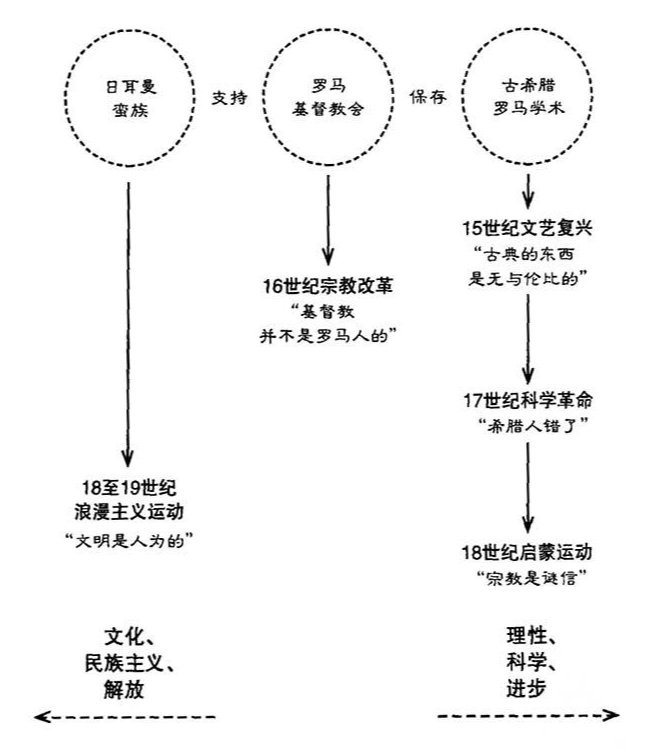
\includegraphics[scale=0.6]{13_1}
				\caption{欧洲历史脉络} 	
			\end{figure}
		\end{enumerate}
	
	\newpage
	
	\section{上帝掷骰子吗}
	
		\centering{曹天元}
	
		\begin{enumerate}
		
			\item 麦克斯韦的理论预言,光其实只是电磁波的一中,这个预言由赫兹在1887年用实验予以了证实。波动说突然发现,它已经不仅仅是光领域的领导者,而是业已成为了整个电磁王国的最高司令官。它的光辉到达了顶点,只要站在大地上,它的力量就像古希腊神话中的巨人那样无穷无尽而不可战胜。它所依靠的大地,就是麦克斯韦不朽的电磁理论。
			
			\item 19世纪末的物理学天空中闪烁着金色的光芒,象征着经典物理帝国的全盛时代。这样的伟大时期在科学史上是空前的,或许也将是绝后的。然而,这个统一的强大帝国却注定了只能昙花一现。喧嚣一时的繁盛,终究要像泡沫那样破灭凋零。
			
			\item 牛顿的体系闪耀着神圣不可侵犯的光辉,从诞生的那刻起便有着一种天上地下唯我独尊的气魄。麦克斯韦的方程组简洁深刻,倾倒众生,被誉为上帝谱写的诗歌。爱因斯坦的相对论虽然是平民出身,但骨子里继承着经典体系的贵族优雅气质,它的光芒稍经发掘后便立刻照亮了整个时代。但量子论却不同,量子论的成长史,更像是一部艰难的探索史,其中的每一步,都充满了陷阱、荆棘和迷雾。量子的诞生伴随着巨大的阵痛,它的命运注定了将要起伏而多舛。量子论的思想是如此反叛,以至于它与生俱来有着对抗权贵的平民风格;而它显示出来的潜力又是如此巨大而近乎无法控制,这一切使得所有人都对它怀有深深的惧意。
			
			\item 如果站在一个比较高的角度看历史,一切事物都是遵循特定的轨迹的,没有无缘无故的事情,也没有不合常理的发展。在时代浪尖弄潮的英雄人物,其实只是适合了那个时代的基本要求,这才得到了属于他们的无上荣耀。
			
			但是如果站在庐山之中,把我们的目光投射到具体的那个情景中去,我们也能够理解一个伟大人物为时代所带来的光荣与进步。虽然不能说,失去了这些伟大人物,人类的发展就会走向歧途,但是也不能否认英雄和天才们为这个世界所作出的巨大贡献。
			
			在科学史上就更是这样。整个科学史可以说就是以天才的名字来点缀的灿烂银河,而有几颗特别明亮的星辰,它们发出的光芒穿越了整个宇宙,一直到达时空的尽头。他们的智慧在某一个时期散发出如此绚烂的辉煌,令人叹为观止。一直到今天,我们都无法找出更加适合的字句来加以形容,而只能冠以“奇迹”之名。
			
			\item 当年被打倒在地的霸主以反叛的姿态再次登上舞台,向已经占据了王位的波动说展开挑战。这两个命中注定的对手终于要进行一场最后的决战,从而领悟到各自存在的终极意义:如果没有了你,我独自站在这里,又是为了什么。
			
			\item 不存在一个客观的、绝对的世界。唯一存在的,就是我们能够观测到的世界。物理学的全部意义,不在于它能够揭示出自然“是什么”,而在于能够明确,关于自然我们能够“说什么”。没有一个脱离于观测而存在的“绝对自然”,只有我们和那些复杂的测量关系,纵横交错,构成了这个宇宙的全部。测量是物理学的核心,测量行为创造了整个世界。
			
			\item 在概率解释,不确定性原理和互补原理这三大核心原理中,前两者摧毁了经典世界的严格因果性,互补原理和不确定性原理又合力捣毁了世界的绝对客观性。
			
			不确定性原理限制了我们对微观世界认识的极限,而这个极限也就是具有物理意义的一切。其次,因为存在着观测者对被观测物体的不可避免的扰动,主体和客体世界必须被理解成一个不可分割的整体。没有一个孤立地存在于客观世界的事物,事实上一个纯粹的客观世界是没有的,任何事物都只有结合一个特定的观测手段,才谈得上具体意义。对象所表现出的形态,很大程度上取决于我们的观测方法。对同一个对象来说,这些表现形态可能是相互排斥的,但必须被同时用于对这个对象的描述中,也就是互补原理。
			
			最后,因为我们的观测给事物带来各种原则上不可预测的扰动,量子世界的本质是“随机性”。传统观念中的严格因果关系在量子世界是不存在的,必须以一种统计性的解释即波函数来取代。
			
			\item 当一个文化衰落之时,曾经为此文化所感之人必感到强烈的痛苦。
			
			\item 任何一种基本量子现象只有在其被记录之后才是一种现象。在光子上路之前还是途中做出决定,这在量子实验中是没有区别的。历史不是确定和实在的——除非它已经被记录下来。
			
			\item 按照MWI(Many Worlds Interpretation),宇宙(Universe)始终只有一个,它的状态可以用一个总体波函数表示,这个波函数严格而连续地按照薛定谔方程演化。但从某一个特定世界(World)的角度来看,则未必如此。波函数随着时间的流逝变得越来越复杂,投影的世界也越来越多,薛定谔方程的每一个可能的解都一定对应了一种投影,因此一切可能发生的事情都在某个“世界”发生了。
			
			MWI认为在双缝干涉实验中必定存在着两个“世界”:左世界和右世界。宇宙态矢量分别在这两个世界中投影为|通过左缝>和|通过右缝>两个量子态。但因为这两个世界维数较低,所以它们两个并不是完全正交的,每个世界都能清晰地“感觉”到另一个世界的投影。这两个世界仍然彼此相干,因此电子能够同时感觉到双缝而自我干涉。
			
			当我们通过仪器观测电子之后,我们就必须谈论“我们发现了电子在左”这样的量子态,它必定存在于一个更大的世界中。“知左”世界描述了电子、仪器和我们本身在内的总体情况,它涉及到了比单个电子多得多的变量、这样一来,“知左”和“知右”世界的维度要比“左”和“右”世界高出不知凡几。在与环境发生复杂的相互纠缠作用之后,我们可以看到,这两个世界戏剧性地变为基本正交而互不干涉。知左世界在知右世界中没有了投影,它们无法彼此感觉到对方了。这个过程被称作“退相干”,量子叠加态在宏观层面上的瓦解,正是退相干的直接后果。
			
			\item 宏观和微观的关键区别,就在于牵涉到维度的不同。这里所说的空间、维度,都是指构造量子态矢量所依存的希尔伯特空间,而非真实时空。事实上,所有的“世界”都存在于同一个物理时空中,只不过它们量子态的映射因为互相正交而无法彼此感受到对方而已。
			
			\item 在隐变量理论中,我们对两个粒子的描述是符合常识的:无论观察与否,两个例子的状态从分裂的一刹那起都是确定无疑的。也就是说,如果世界的本质是经典的:1.定域的,没有超过光速信号的传播;2.实在的,存在一个独立于我们观察的外部世界,那么我们任意取3个方向观测两个粒子的自旋,它们所表现出的协作程度必定要受限于贝尔不等式。
			
			\item 路径积分是一种对于空间和时间求和的方法:当粒子从A运动到B,它并不具有经典理论中所描述的那样一个确定轨道。相反,我们必须把它的轨迹表达为所有可能的路径的叠加。在路径积分的计算中,我们只关心粒子的初始状态和最终状态,而完全忽略它的中间过程。对于这些我们不关心的事情,我们简单地把它在每一种可能的路径上遍历求和,精妙的是,最后大部分路径往往会自相抵消,只剩下那些为量子力学所允许的轨迹。
			
			按照退相干历史(DH)的解释,假如我们把宇宙的历史分得足够精细,那么实际上每时每刻都有许许多多的精细历史在“同时发生”(相干)。但一般来说,我们对于过于精细的历史没有兴趣,我们只关心我们所能观测到的粗略历史的情况。因为退相干的原因,这些历史之间失去了联系,只有一种能被我们感知到。
			
			如果DH理论是正确的,那么我们每时每刻其实都经历着多重的历史,世界上的每一个粒子,事实上都处在所有可能的历史的叠加中。但一旦涉及到宏观物体,我们所能够观测到则无非是一些粗略化的历史,当细节被抹去时,这些历史便互相退相干,永久地失去了联系。
			
			\item 在量子场论中,所有粒子都是弥漫在空间中的某种场,这些场有着不同的能量形态,当能量最低时,就是我们所说的“真空”。因此真空其实不过是粒子的基态而已,任何粒子都可以从中被创造出来,也可以互相湮灭。
			
			\item 在超弦理论中,任何粒子其实都不是传统意义上的点,而是开放或闭合的弦。当它们以不同的方式振动时,就分别对应于自然界中的不同粒子(电子、光子、引力子等等)。我们仍然生活在一个10维的空间里,但是有六个维度是紧紧蜷缩起来的,所以平时察觉不到。这6个蜷缩的维度不停地扰动,从而造成了全部的量子不确定性。
			
			M理论中,时空变成了11维,由此可以衍生出所有5种10维的超弦论,事实上,由于多了一维,另有一个超引力的变种。时空的基本结果可能是从0维到9维的任意维数。
			
			\item 或许历史终究是一场轮回,但在每一次的轮回中,我们毕竟都获得了更伟大的发现。科学在不停地检讨自己,这这种谦卑的审视和自我否定不但没有削弱它的荣光,反而使它获得了永恒的力量,也不断增强着我们对于它的信心。人类居住在太阳系的一颗小行星上,他们的文明不过万年的历史,现代科学的创立不到400年。但他们的智慧贯穿整个时空,从最小的量子到最大的宇宙尺度,从大爆炸的那一刻到时间的终点,从最近的白矮星到最远的宇宙视界,没有什么可以阻挡我们探寻的脚步。这一切,都来自于我们对成功的信念,对于科学的依赖,以及对于神奇的自然那永无休止的好奇。	
			
		\end{enumerate}

	\newpage
	
	\section{时间简史}
	
		\centering{史蒂夫·霍金}
		
		\begin{enumerate}
			\item 一个好的理论的特征是,它能给出许多原则上可以被观测所否定或证伪的预言。
			
			\item 假定我们是有理性的生物,既可以随意自由地观测宇宙,又可以从观测中得出逻辑推论。在这样的方案里可以合理地假设,我们可以越来越接近到制约我们宇宙的定律。但是如果真有一套完整的统一理论,则它也将决定我们的行动。这样理论本身将决定我们对之探索的结果。那么为什么它必须确定我们从证据中得到正确的结论?它不也可以确定我们得到错误的结论吗?或者根本没有结论?
			
			依据达尔文的自然选择原理,在自繁殖群体中,存在不同个体在遗传物质和发育上的差异,某些个体比其他个体对周围的世界更能引出正确的结论,并去适应它。这些个体更可能存活、繁殖,因此它们的行为和思维模式将越来越起到主导作用。假定宇宙已经以规则的方式演化至今,我们可以预期,自然选择赋予我们的推理能力在探索完整统一理论时仍然有效,并因此不会导致我们得到错误的结论。
			
			\item 当一个物体运动时,或者当一个力起作用时,它影响了空间和时间的曲率;反过来,时空的结构影响了物体的运动和力作用的方式。空间和时间不仅去影响、而且被发生在宇宙中的每一件事所影响。
			
			\item 在量子力学中,所有物质粒子之间的力或者相互作用都被认为是由自旋为整数0、1、2的粒子承担。自旋数为1/2的物质粒子——譬如电子或夸克——发出携带力的粒子,由于发射粒子引起的反弹,改变了物质粒子的速度。携带力的粒子又和另一物质粒子碰撞而被吸收。这碰撞改变了第二个粒子的速度,正如同两个物质粒子间存在过一个力。
			
			\item 时间箭头将过去和未来区别开来,使时间有了方向。至少有三种不同的时间箭头:第一个,是热力学时间箭头,即在这个时间方向上无序度或者熵增加;第二个是心理学时间箭头,这就是我们感觉时间流逝的方向;最后是宇宙学时间箭头,在这个方向上宇宙在碰撞而不是收缩。
			
		\end{enumerate}
	
	\newpage
	
	\section{中国哲学简史}
	
		\centering{冯友兰}
		
		\begin{enumerate}
			\item 中国哲学以为,一个人不仅在理论上而且在行动上完成出世和入世的统一,就是圣人。中国圣人的精神成就,相当于佛教的佛、西方宗教的圣者的精神成就。但是中国的圣人不是不问世务的人。他的人格是所谓的“内圣外王”的人格。“内圣”是就其修养的成就说;“外王”是就其在社会上的功用说。圣人不一定有机会成为实际政治的领袖。只是说,有最高的精神成就的人,按道理可以为王,而且最宜为王。至于实际上他是否有机会为王,无关宏旨。
			
			\item 学哲学的目的,是使人作为人能够成为人,而不是成为某种人。
			
			\item 任何时代或者任何民族的哲学,总有一部分只相当于那个时代或者那个民族具有价值,但总有另一部分比这种价值更大一些。
			
			\item 儒家者流盖出于文士,墨家者流盖出于武士,道家者流盖出于隐者,名家者流盖出于辩者,阴阳家者流盖出于方士,法家者流盖出于法术之士。
			
			\item 如何实行仁,在于推己及人。“己欲立而立人,己欲达而达人”,己之所欲,亦施于人,这是推己及人的肯定方面,孔子称为“忠”,即“尽己为人”。推己及人的否定方面,孔子称之为恕,即“己所不欲,勿施于人”。推己及人的两个方面合在一起,就叫做忠恕之道,即为“仁之方”。
			
			\item 忠恕之道同时就是仁道,行忠恕就是行仁。行仁就必然履行在社会中的责任和义务,这就包括了义的性质。因而忠恕之道就是人的道德生活的开端和终结。
			
			\item 知命也就是承认世界本来存在的必然性。这样对于外在的成败也就无所萦怀。
			
			\item 墨家相信鬼神存在,可是同时反对丧葬和祭祀的缛礼,固然好像是矛盾的。儒家强调丧礼和葬礼,可是并不相信鬼神存在,同样也好像是矛盾的。
			
			儒家、墨家这些好像是矛盾的地方,都不是真正的矛盾。照儒家所说,行祭礼的原因不再是因为相信鬼神真正存在,当然相信鬼神存在无疑是祭礼的最初原因。行礼只是祭祀祖先的人出于孝敬祖先的感情,所以礼的意义是诗的,不是宗教的。同样在墨家的观点中也没有实际的矛盾。因为墨子要证明鬼神存在,本来就是为了给他的兼爱学说设立宗教的制裁,并不是对于超自然的实体有真正的兴趣。他的“天志”、“明鬼”不过是诱导人们相信:实行兼爱则赏,不实行兼爱则罚。在人心之中有这样一种信仰也许是有用的,因此墨子需要它。“节用”、“节葬”也是有用的,因此墨子也需要它。从墨子的极端功利主义观点来看,需要这两种东西是毫不矛盾的,因为两者都是有用的。
			
			\item 《韩非子》说杨朱“不以天下大利易其胫一毛”,与《孟子》说杨朱“拔一毛而利天下,不为也”,有些不同。可是这两种说法与杨朱的基本观念是一致的。前者与“轻物重生”一致,后者与“为我”一致。
			
			\item 道家的哲学出发点是全生避害。为了全生避害,杨朱的方法是“避”,逃离人世,遁迹山林,心想这样就可以避开人世的恶。可是人世间的事情多么复杂,不论你隐藏得多好,总是有些恶仍然无法避开。
			
			老子的大部分思想表示出另一种企图,就是揭示宇宙事物变化的规律。事物变,但是事物变化的规律不变。一个人如果懂得了这些规律,并且遵循这些规律调整自己的行动,就能够使事物转向对他有利。这是先秦道家发展的第二阶段。
			
			可是事物的变化中总有些没能预料到的因素。老子把话说穿:“吾所以有大患者,为吾有身,及吾无身,吾有何患!”这种大彻大悟之言,《庄子》有许多地方加以发挥,产生了“齐生死、一物我”的理论。它的意思是,从一个更高的观点看生死、物我,超越现实的世界,不是从社会到山林,而像是从这个世界到另一个世界。这是先秦道家发展的第三阶段,也是最后一个阶段。
			
			\item 孟子认为,人之所以异于禽兽,在于有人伦以及建立在人伦之上的道德原则。国家和社会起源于人伦。照墨家所说,国家的存在是因为它有用;照儒家说,国家的存在是因为它应当存在。
			
			\item 惠施强调实际事物是可变的、相对的这个事实,公孙龙则强调名是不变的、绝对的这个事实。
			
			\item 名家的哲学家通过分析名,分析名与实的关系或者区别,发现了中国哲学中称为“超乎形象”的世界。在中国哲学中,有“象内”“象外”的区别。在形象之内者,是“实”。譬如大小方圆,长短黑白,都是一种形象。凡可为某种经验的对象,或某种经验的可能的对象者,都是有形象的,也可以说是,都是在形象之内的,都存在于实际世界之内。反过来说,凡是有形象的,在形象之内的,存在于实际世界之内的,都是某种经验的对象,或其可能的对象。
			
			\item “无名天地之始。”这个命题只是一个形式的命题,不是一个积极的命题。就是说,它对于实际没有任何肯定。既然有万物,必有万物之所从生者。这个“者”,他们起个代号叫做“道”,“道”其实不是名。“道”的概念也是一个形式的概念,不是一个积极的概念。这个概念,对于万物之所从生者是什么,其实什么也没有说。能够说的只有一点,就是,既然“道”是万物之所从生者,它必然不是万物中之一物。因为它若是万物中之一物,它就不能同时是万物之所从。每类物都有一名,但是“道”本身不是一物,所以它“无名,朴”。
			
			\item 老子警告我们:“不知常,妄作,凶。”我们应该知道自然规律,根据它们来指导个人的行动。老子把这叫做“袭明”。人“袭明”的通则是,想要得到些东西,就要从反面开始;想要保持些什么东西,就要在其中容纳一些与之相反的东西。“不自见,故明。不自是,故彰。不自伐,故有功。不自矜,故长。夫唯不争,故天下莫能与之争。”这说明了通则的第一点。“大成若缺,其用必弊。大盈若冲,其用不穷。大直若屈。大巧若拙。大辩若讷。”又说:“曲则全。枉则直。洼则盈。敝则新。少则得。多则惑。”这说明了通则的第二点。
			
			\item 老子认为,道生万物。在这个生的过程中,每个个别事物都从普遍的道中获得一些东西,这就是“德”。“德”意指power(力)或virtue(德)。“德”可以是道德的,也可以是非道德的,一物自然地是什么,就是它的德。老子说:“万物莫不尊道而贵德。”这是因为,道是万物之所从生者,德是万物之所以是万物者。
			
			道是万物之所以生者。道本身不是一物,所以它不能像万物那样“为”。可是万物都生出来了。所以道无为而无不为。道,让每物做它自己能做的事。
			
			\item 庄子认为,获得幸福有不同等级。自由发展我们的自然本性,可以使我们获得一种相对幸福;绝对幸福是通过对事物的自然本性有更高一层的理解而得到的。
			
			万物的自然本性不同,其自然能力也各不相同,可是有一点是共同的,就是在它们充分而自由地发挥其自然能力的时候,它们都是同等的幸福。
			
		    圣人对万物的自然本性有完全的理解,所以无情。但是并不是说圣人没有感情。这宁可是说,他不为情所忧乱,而享有所谓“灵魂的和平”。如斯诺宾莎所说:“无知的人不仅在各方面受到外部原因的扰乱,从未享受灵魂的真正和平,而且过着对万物似乎一概无知的生活,活着也是受苦,一旦不再受苦了,也是不再存在了。另一方面,有知的人,在他有知的范围内,简直可以不动心,而且由于他理解自己、万物都有一定的永恒的必然性,他也就永远存在,永远享受灵魂的和平。”圣人由于对万物自然本性有理解,他的心就再也不受世界变化的影响。用这种方法,他就不以来外界事物,因而他的幸福也不受外界事物的限制,他可以说是得到了绝对幸福。
		
			道家思想还有一个方向,它强调万物自然本性的相对性,以及人与宇宙的同一。要达到这种“同一”,人需要更高层次的知识和理解。由这种同一所得到的幸福才是真正的绝对的幸福。
			
			\item 在是与非的对立中,像一个循环无尽的圆。但是从道的观点看事物的人,好像是站在圆心上。他理解在圆周上运动着的一切,但是他自己则不参与这些运动。这不是由于他无所作为,听天由命,而是因为他以及超越有限,从一个更高的观点看事物。
			
			\item "至大无外,谓之大一。"由于“大一”无外,所以它是不可思议、不可言说的。因为任何事物,只要可以思议、可以言说,就一定有外,这个思议、言说就在它本身以外。
			
			\item “无知”与“不知”不同。“无知”状态是原始的无知状态,而“不知”状态则是先经过有知的阶段后才达到的。前者是自然的产物,后者是精神的创造。
			
			\item   后期墨家遵循墨子功利主义哲学的传统,主张人类的一切行为的目的在于取利避害。他们都认为“义,利也”。利是义的本质。但是什么是利的本质?《经上》说:“利,所得而喜也。”“害,所得而恶也。”这也后期墨家就位墨家的功利哲学做出享乐主义的解释。边沁说:“功利哲学即承认人类服从快乐与痛苦二威权之事实,而以之为哲学的基础。此哲学之目的,在以理性、法律维持幸福。”照他的说法,道德的目的就是“最大多数的最大幸福”。
			
			\item 照孟子所说,仁义礼智这“四端”是天生的,只要充分发展这四端,人就成为圣人。但是照荀子所说,人不仅生来毫无善端,相反倒是具有实际的恶端。但是他也肯定,除了恶端,人同时还有只能,可以使人向善。孟子说“人皆可以为尧舜”,是因为人本来是善的;荀子论证“涂之人可以为禹”,是因为人本来是智的。
			
			\item 人必须先说很多话,然后保持静默。
			
			
		\end{enumerate}
	
	\newpage
	
	\section{人类群星闪耀时}	
			
		\centering{斯蒂芬·茨威格}	
			
		\begin{enumerate}
			
			\item 历史大部分时候是个编年史家,他冷漠而持久地穿针引线,将那根巨大的历经千年的链条环环相连,因为所有的巅峰时刻需要绸缪,所有非凡之事需要酝酿。一个民族,总是上百万人中才涌现出一位天才。世界总是在荒芜了漫长的无谓时光后,真正的历史性时刻,人类群星闪耀的时刻才悉数登场。
			
			\item 西班牙征服者的性格和行为中混杂着难以解释的特质。一方面他们在炙热的灵魂深处,以在那个时代唯有基督徒才具有的虔诚呼唤上帝,一方面又以上帝之名书写耻辱而灭绝人性的历史。他们一面以勇气、牺牲精神和耐受力创造着神圣的英雄业绩,一面又以不知羞耻的方式尔虞我诈。他们以卑鄙铸造尊严,铸造伟大而真正值得称颂的历史使命感。
			
			\item 穆罕默德想出了一个绝妙的主意。他打算让他的船队从无人的外海出发,穿过岬角,抵达金角湾内港。这一令人震惊的大胆想法——把上百条船拖过多山的岬角地带,听起来如此荒谬不可实现,以致拜占庭人和热内亚人不可能想到会有这样的战略部署,就像他们之前的罗马人和他们之后的奥地利人不会想到汉尼拔和拿破仑的人马能迅速越过阿尔卑斯山一样。按常理,船队只能航行在水面上,不可能翻越高山。然而把不可能变为可能才是魔鬼般意志的真正标志。从这一标志中,人们总能认出一位嘲弄军事规则的军事天才。这些天才会在适当的时候以具有创造性的临场发挥取代循规蹈矩。
			
			\item 黑暗中,烛光卖力地同低垂的穹顶扭打着,照耀着跪在地上垂死挣扎的黑压压宛如一整具躯体的人群。这具巨大的躯体是拜占庭的灵魂,它正向上帝祈祷。大主教提高了声音的高度和力度领诵着,唱经班随声附和。堂内再次响起西方世界神圣而永恒的声音——音乐。接着,皇帝打头,一个人接着一个人走到祭台前领受天主的慰藉,直至不绝的祈祷直达天庭,在巨大的教堂内回荡。这是东罗马帝国最后一次安魂弥撒。在这座查士丁尼建造的主教堂内,这将是最后一次基督教礼程仪式。
			
			\item 首演时的《马赛曲》尚未真正显示它的力量。它不是为抒情男高音创造的演示作品,也不适合某位歌手在小资产阶级沙龙里,夹在浪漫曲和意大利咏叹调之间演唱。《马赛曲》是一首节奏强劲有力、激越昂扬的战歌。“公民们,武装起来!”应当唱向民众,唱向人群,而真正的配器应该是叮当的武器声。它不是为那些正襟危坐的欣赏者,而是为拥有共同志向,准备共同战斗的人而作。它是为千人合唱而作,它是一首杰出的进行曲、凯旋曲、祖国颂,是全体人民的国歌。
			
			\item 尘世间,这样的瞬间极少光顾,而当它降临到一个不恰当的身上时,这人并不懂得如何利用它。于是,这一伟大的瞬间进行了可怕的复仇。一切市民的美德:谨慎、顺从、勤勉、深思熟虑,在天命降临的烈焰中化为乌有,百无一用。这一刻需要天才。它蔑视地将胆怯之人一把推开并将天才一举锻造为不朽的丰碑。这世上的另一位神,命运,它高举勇者,以火热的双臂将英雄们举向天国。
			
			\item 要想成就一个奇迹或者一项伟业,一个重要的前提不可或缺:对这一奇迹深信不疑。执着者的天真和勇气,往往能富有创造性地促进学者们迟迟不进的计划。
			
			\item 最后这萧索而低微的命运无损于他的伟大。假如列夫·托尔斯泰不为他人受苦,今天他就不会属于全人类。
			
			\item 看上去徒劳无功的事业再次结出硕果,遗憾的事业变为向人类的大声疾呼:将力量集中起来吧,挑战那些尚未抵达的目的地。伟大的对决中,英雄虽死犹生,失败中的意志崛起,直抵无限高峰。因为偶然的成功和轻易的胜利只能点燃人的虚荣之心,却不能获得一个人在与不可战胜的强大命运的搏击中,因为覆灭而升华的高尚心灵。这类一切时代,一切悲剧中最伟大的杰作,时常刻画于诗人笔下又千百次地在生活中诞生。
			
			\item 然而历史不断上演着这样的悲剧:智者们往往因为内心肩负着巨大的责任,而在重要时刻优柔寡断。这种内心的矛盾冲突不断表现在拥有智慧和创造性的人身上:他们比别人更能认清时代的蠢行,他们亦卷入时代的浪潮,亦会在狂热的激情中投身到政治斗争中;同时,他们又会踌躇于以暴制暴的行径。而这种犹疑和顾虑恰恰在那些要求他们铤而走险的时刻令他们丧失了行动力量。 
			
		\end{enumerate}
		
	
	\newpage
	
	\section{Das Kapital}
	
		\centering{Karl Marx}
		
		\begin{enumerate}
			\item Der Reichtum der Gesellschaften,in welchen kapitalistische Produktionsweise herrscht, erscheint als eine ungeheure Warensammlung, die einzeln Ware als seine Elementarform.
			
			\item Jedes nützliche Ding, ist unter doppelten Gesichtspunkt zu betrachten,nach Qualität und Quantität. Als Gebrauchswert sind die Waren vor allem verschiedener Qualität, als Tauschwert können sie nur verschiedener Quantität sein, enthalten also kein Atom Gebrauchswert.
			
			\item Es ist nur das Quantum gesellschaftlich notwendiger Arbeit oder die zur Herstellung eines Gebrauchswerts gesellschaftlich notwendiger Arbeitszeit, welche seine Wertgröße bestimmt.
			
			\item Nur Produkte selbständiger und voneinander unabhängiger Privatarbeiten treten einander als Waren gegenüber.
			
		
			
		\end{enumerate}
	
	\newpage
		
	\section{文心雕龙}
	
		\centering{刘勰}
		
		\begin{enumerate}
			\item  文之为德也大矣,与天地并生者何哉?夫玄黄色杂,方圆体分,日月叠璧,以垂利天之象;山川焕绮,以铺理地之行:此盖道之文也。仰观吐曜,俯察含章,高卑定位,故两仪既生矣,唯人参之,性灵所钟,是谓三才,为五行之秀,实天地之心。心生而言立,言立而文明,自然知道也。傍及万品,动植皆文:龙凤以藻绘呈瑞,虎豹以炳蔚凝姿;云霞雕色,有逾画工之妙;草木贲华,无待锦匠之奇。夫岂外饰,盖自然耳。至于林籁结响,调如竽瑟;泉石激韵,和若球锽。故形立则章成矣,声发则文生矣。夫以无识之物,郁然有彩;有心之器,其无文欤?
			
			\item 夫鉴周日月,妙极几神;文成规矩,思合符契。或简言以达旨,或博文以该情,或明理以立体,或隐义以藏用。故《春秋》一字以褒贬,丧服举轻以包重,此简言以达旨也。《邠诗》联章以积句,《儒行》缛说以繁辞,此博文以该情也。书契决断以象夬,文章昭晰以象离,此明理以立体也。四象精义以曲隐,五例微辞以婉晦,此隐义以藏用也。
			
			\item 隐也者,文外之重旨者也;秀也者,篇中之独拔者也。隐以复义为工,秀以卓绝为巧。
			
			彼波起辞间,是谓之秀。纤手丽音,宛乎逸态,若远山之浮烟霭,娈女之靓容华。然烟霭天成,不劳于妆点;容华格定,无待于裁熔;深浅而各奇,秾纤而俱妙,若挥之则有余,而揽之则不足矣。
			
			夫立意之士,务欲造奇,每驰心于玄默之表;工辞之人,必欲臻美,恒匿思于佳丽之乡。呕心吐胆,不足语穷;锻岁炼年,奚能喻苦?故能藏颖词间,昏迷于庸目;露锋文外,惊绝乎妙心。
			
			\item 夫文心者,言为文之用心也。昔涓子《琴心》,王孙《巧心》,心哉美矣,故用之焉。古来文章,以雕缛成体,岂取驺奭之群言雕龙也。夫宇宙绵邈,黎献纷杂,拔萃出类,智术而已。岁月飘忽,性灵不居,腾声飞实,制作而已。夫肖貌天地,禀性五才,拟耳目于日月,方声气乎风雷,其超出万物,亦已灵矣。形同草木之脆,名逾金石之坚,是以君子处世,树德建言,岂好辩哉,不得已也。
		\end{enumerate}
		
	\newpage
	
	\section{韩非子}
	
		\centering{韩非}
		
		\begin{enumerate}
			\item 以至智说至圣,未必直而见受,伊尹说汤是也;以智说愚必不听,文王说纣是也。
			
			愚者难说也,故君子难言也。且至言忤于耳而倒于心,非圣贤莫能听。
			\item 君无见其所欲,君见其所欲,臣自将雕琢;君无见其意,君见其意,臣自将表异。
			
			明君之道,使智者尽其虑,而君因以断事,故君不穷于智;贤者敕其材,君因而任之,故君不穷于能;有功则君有其贤,有过则臣任其罪,故君不穷于名。是故不贤而为贤者师,不智而为智者正。
			
			群臣陈其言,君以其言授其事,事以责其功。功当其事,事当其言,则赏;功不当其事,事不当其言,则诛。
			诚有功,则虽疏贱必赏;诚有过,则虽近爱必诛。疏贱必赏,近爱必诛,则疏贱者不怠,而近爱者不骄也。
			\item 君以其言授之事,专以其事责其功。功当其事,事当其言,则赏;功不当其事,事不当其言,则罚。故群臣其言大而功小者则罚,非罚其小功也,罚功不当名也;群臣其言小而功大者亦罚,非不说于大功也,以为不当名也害甚于有大功,故罚。昔者韩昭侯醉而寝,典冠者见君之寒也,故加衣于君之上,觉寝而说,问左右曰:“谁加衣者?”左右对曰:“典冠”。君以兼罪典衣与典冠。其罪典衣,以为失其事也;其罪典冠,以为越其职也。非不恶寒也,以为侵官之害甚于寒。
			\item 臣主之利相与异者也,何以明之哉?曰:主利在有能而任官,臣利在无能而得事;主利在有劳而爵禄,臣利在无功而富贵;主利在豪杰使能,臣利在朋党用私。是以国地削而私家富,主上卑而大臣重。
			\item 凡说之难:在知所说之心,可以吾说当之。所说出于为名高者也,而说之以厚利,则见下节而遇卑贱,必弃远矣。所说出于厚利者也,而说之以名高,则见无心而远事情,必不收矣。所说阴为厚利而显为名高者也,而说之以名高,则阳收其身而实疏之;说之以厚利,则阴用其言显弃其身矣。
			\item 故舆人成舆,则欲人富贵;匠人成棺,则欲人之夭死也。非舆人仁而匠人贼也,人不贵,则舆不售;人不死,则棺不买。情非憎人也,利在人之死也。
			\item 公孙鞅曰:“行刑重其轻者,轻者不至,重者不来,是谓以刑去刑也。”
			\item 夫良药苦于口,而智者劝而饮之,知其入而已己疾。忠言拂于耳,而明主听之,知其可以致功也。
			\item 有度难而无度易也。有常仪的,则羿、逄蒙以五寸为巧;无常仪的,则以妄发而中秋毫为拙。故无度而应之,则辩士繁说;设度而持之,虽智者犹畏失也,不敢妄言。
			\item 故人行事施予,以利之为心,则越人易和;以害之为心,则父子离且怨。
			\item 小信成则大信立,故明主积于信。赏罚不信则禁令不行、
			\item 不在所与居,在所与谋也。
			\item 利所禁,禁所利,虽神不行;誉所罪,毁所赏,虽尧不治。
			\item 外举不避仇,内举不避子。
			\item 国者,君之车也;势者,君之马也。夫不处势以禁诛擅爱之臣,而必德厚以与天下齐行以争民,是皆不乘君之车,不因马之利,舍车而下走者也。
			\item 申子曰:“独视者谓明,独听者谓聪。能独断者,故可以为天下主。”
			\item 治强生于法,弱乱生于阿,君明于此,则正赏罚而非仁下也。爵禄生于功,诛罚生于罪,臣明于此,则尽死力而非忠君也。君通于不仁,臣通于不忠,则可以王矣。
			\item 以身为苦而后化民者,尧、舜之所难也;处势而矫下者,庸主之所易也。将治天下,释庸主之所易,道尧舜之所难,未可与为政也。
			\item 慎子曰:飞龙乘云,腾蛇游雾,云罢雾霁,而龙蛇与蚓蚁同矣,则失其所乘也。尧为匹夫,不能治三人;而桀为天子,能乱天下:吾以此知势位之足恃而贤智之不足慕也。
			
				  应慎子曰:夫有云雾之势而能乘游者,龙蛇之材美也;今云盛而蚓弗能乘也,雾醲而蚁不能游也,夫有盛云醲雾之势而不能乘游者,蚓蚁之材薄也。
				  
				  复应之曰:夫贤之为道不可禁,而势之为道也无不禁,以不可禁之贤与无不禁之势,此矛盾之说也。
				  
				  世之治者不绝于中,吾所以为言势者,中也。中者,上不及尧舜,而下亦不为桀纣。抱法处势则治,背法去势则乱。
			\item 是以圣人不期修古,不法常可,论世之事,因为之备。
			\item 故圣人议多少、论厚薄为之政。故罚薄不为慈,诛严不为戾,称俗而行也。故事因与世,而备适于事。
			\item 是以赏莫如厚而信,使民利之;罚莫如重而必,使民畏之;法莫如一而固,使民知之。
			\item 儒以文乱法,侠以武犯禁,而人主兼礼之,此所以乱也。
			\item 国平养儒侠,难至用介士,所利非所用,所用非所利。
			\item 故明主之国,无书简之文,以法为教;无先王之语,以吏为师;无私剑之悍,以斩首为勇。是境内之民,其言谈者必轨于法,动作者归之于功,为勇者尽之于军。是故无事则国富,有事则兵强,此之谓王资。
			\item 鄙谚曰:长袖善舞,多钱善贾。此言多资之易为功也。故治强易为谋,弱乱难为计。故用于秦者,十变而谋稀失,用于燕者,一变而计希得。非用于秦者必智。用于燕者必愚也,盖治乱之资异也。
			\item 无参验而必之者,愚也;弗能必而据之者,诬也。
			
		\end{enumerate}
	
	
	\newpage
	
	\section{动物庄园}
	
		\centering{乔治·奥威尔}
		
		\begin{enumerate}
			\item 同志们!难道你们认为,我们猪这样做是自私自利和享受特权的一种表现?我们有许多同志其实讨厌苹果和牛奶。我自己就讨厌他们。我们食用这些东西的唯一目的就是保持我们的身体健康。牛奶和苹果(同志们,这都是科学证明了的)含有一口猪保持身体健康不可或缺的物质。我们猪是脑力劳动者。本农场的整个管理部门全都依靠我们。我们白天黑夜都在守护着你们的福祉。正是为了你们,我们才喝那些牛奶,吃那些苹果。要是我们这些猪无法尽责,你们可知道会发生什么?琼斯将会回来!是的,琼斯将会回来!同志们,想必你们当中没有谁愿意看到琼斯回来吧?
			
			\item 如果说紫苜蓿在心中为自己设计过什么关于未来的蓝图的话,那幅蓝图上将是一个摆脱了饥饿和鞭子的动物社会,大家一律平等,工作各尽所能,强者卫护弱者,就像在听少校演讲之夜紫苜蓿用她的前腿卫护一窝失恃的小鸭那样。可是,理想的动物社会没有盼到,而他们反倒落入了这样一个时代:谁也不敢说出自己的想法,动辄狂吠不止的恶犬到处横行,你不得不眼睁睁看着你的同志在招认了丑恶罪行后被撕成碎片——她不知道怎么会闹成这样的。她头脑里并没有造反或违命的想法。她知道,即使就目前的状况而言,他们的日子仍然比琼斯时代好得多。她也知道,必须阻止人们卷土重来——这比其他一切更重要。不管发生什么事情,她将保持忠诚,努力工作,完成交给她的任务,接受拿破仑的领导。可是,说到底,她和所有别的动物希望看到并为之埋头苦干的,毕竟不是现在这种局面。他们建造风车,横眉冷对琼斯的猎枪子弹,也不是为了过今天这样的日子。这便是她的想法,尽管她缺乏言语把想法表达出来。
			
			\item 吱嘎的解释是,口粮问题上缺乏灵活性的平均主义做法是与动物主义的原则背道而驰的。在任何情况下,他都能轻而易举地向别的动物证明,他们的食物实际上并不短缺,不管表面上看起来如何。眼下嘛,当然喽,发现有必要对口粮标准做一些调整(吱嘎永远称这是“调整”,而绝对不说“削减”),但与琼斯时代相比,还是大有改善。他用高频率的尖嗓音飞快地读出一大串数字,不厌其详地向他们证明,他们比琼斯时代拥有更多燕麦,更多干草,更多圆萝卜,他们的工作时间缩短了,他们饮用水的水质提高了,他们的寿命更长了,他们的后代成活率更高了,他们圈栏里的干草更多了,受跳蚤的滋扰减少了。动物们相信,这些话句句都是事实。说真的,琼斯以及琼斯所代表的一切,几乎已经从动物们的记忆中淡出了。他们知道,当前的生活十分艰苦,简直难以糊口,他们时常感到饥饿,时常感到寒冷,他们通常除了睡觉就是干活。不过往昔的日子更苦,这是毫无疑问的。他们乐于相信这样的说法。此外,在往昔的日子里他们是奴隶,而现在他们是自由的,那才是最根本的区别——吱嘎决不会忘了指出这一点。
			
			\item 如今墙上只有一条戒律,其余什么都没有。那唯一的一诫是:凡动物一律平等,但是有些动物比别的动物更平等。
			
			\item 十二条嗓门暴跳如雷地吼叫,声音全都一个样。这下弄明白了,猪的脸究竟出了什么问题。动物们从窗外往里望,目光从猪移到人,再从人移到猪,又重新从猪移到人,要分清哪张脸是猪的,哪张脸是人的,已经不可能了。
			
		\end{enumerate}
	
	\newpage
	
		\section{美丽新世界}
		
			\centering{奥尔德斯·赫胥黎}
			                                                       231 235 289
			\begin{enumerate}
				\item 标准化的男人和女人,标准化的群体。一个小型工厂的员工可能就是同一个波卡诺夫斯基流程处理的卵子的产物。
				
				“九十六个一模一样的多胞胎操作九十六部一模一样的机器!”他的声音几乎因为兴奋而发颤。“现在你们知道自己置身于何处了。历史上第一次,”他引用了世界观的格言,“集体、身份、稳定。”多么伟大的言论。如果我们能将波卡诺夫斯基流程无限制进行下去的话,所有的问题都将得以解决。
				
				\item “你知道那是什么样的过山车吗?”他说道,“是某个人最终消失无痕,变成一股升腾的热气。我很好奇,想知道那会是谁——男人还是女人,阿尔法还是埃普斯隆……”他长叹一声,然后以坚定而热情的语气总结道:“不管怎样,有一件事情我们可以肯定:无论他是谁,当他活着的时候他很开心。现在每个人都很开心。”
				
				“是的,现在每个人都很开心。”莱妮娜跟着说了一遍。这句话他们俩每天晚上要重复听一百五十遍,一直听了十二年。
				
				\item “我想要体验某种强烈的东西。”
				\\ “当个体感知时,集体就会动摇。”
				\\ “嗯,那为什么就不能让它稍微动摇呢?”
				
				\item “我们的信仰是幸福和稳定。只由阿尔法组成的社会一定是动荡和悲惨的社会。想象一个工人都是阿尔法的工厂,也就是说,那些工人都是独立的没有关系的个体,有优秀的天赋,而且所接受的培育是能够做出自由的选择和承担责任(在有限范围内)。”
				\\ “那很荒谬。一个接受阿尔法的试管培育和教育的人,如果得去做半痴呆的埃普斯隆做的工作,他会发疯的。阿尔法能完全实现社会化——但前提是你让他们承担阿尔法的工作。只有埃普斯隆能够作出埃普斯隆式的牺牲,原因很简单,对于他来说,那并不是牺牲,他们不会和你作对。他所接受的培育规定了他必须遵循的轨道。他只能这么做,他的命运已经注定好了。即使出瓶后,他仍然困在一个瓶子里——一个看不见的按照胚胎期和婴儿期的固定模式行事的瓶子里。”主宰若有所思地继续说道,“当然,我们每个人这辈子都在瓶子里度过。但如果我们是阿尔法,我们的瓶子相对来说是很广阔的。如果我们被局限在一个狭窄的空间里的话,我们会觉得非常痛苦。你不能将为上等人准备的人造香槟倒入下层阶级的瓶子里。”
				
				\item “我喜欢那些麻烦。”
				\\ “我们不喜欢。”主宰者说道,“我们希望过得很舒适。”
				\\ “我不要舒适。我要上帝,我要诗歌,我要真正的危险,我要自由,我要美好,我要罪恶。”
				\\ “事实上,你要求的是不幸福的权利。”
				\\ “那好吧。”野人轻蔑地说道,“我正是在要求不幸福的权利。”
				
				\item 我们这个时代的梦魇源于没有秩序,而《美丽新世界》的梦魇源于过度秩序化。  
				
				\item 在《美丽新世界》里,我所幻想的优生学和劣生学得以系统实现。在一组瓶子里装着生理质量优秀的卵子,由生理质量优秀的精子进行受精,得到最好的产前处理,最后通过试管培育出贝塔、阿尔法甚至优等阿尔法。在另一组数量多得多的瓶子里,生理质量低劣的卵子由生理质量低劣的精子受精,然后接受波卡诺夫斯基流程处理(由一个卵子培育出九十六个一模一样的多胞胎),并在产前再用酒精和其他蛋白质毒素加以处理。这些通过试管培育出的生物几乎算不上人,但是他们能够进行非技术性的工作,经过适当的培育,自由频繁地与异性交往以放松身心,沉溺于免费的娱乐消遣,并通过每日服用苏摩对良好的行为模式加以强化,不会为他们的上司制造麻烦。
				
				\item 组织是不可或缺的,因为只有在一个由自由合作的个体组成的实行自我管理的社区内,自由才能存在和拥有意义。但是,尽管不可或缺,组织也可能是致命的。过度的组织会将男人和女人变成自动机器,扼杀创新精神和毁灭自由存在的可能。唯一的安全途径是在自由放任和完全控制这俩个极端之间找到一条中庸之道。
				
				\item 个体必须由充分的暗示感受性,愿意并且能够使社会运转,但不能有过分的暗示感受性,以免无助地落入职业思想操纵者的圈套。同样地,他们应该接受关系分析宣传内容的充分的指导,不至于不加批判地相信胡说八道的内容,但不能有过度的批判性,让他们断然拒绝并非总是符合理性的出于善意的传统守护者所说的话。
			
			\end{enumerate}
	\newpage
	
	\section{东周列国志}
		\centering{冯梦龙}
		\begin{enumerate}
			\item 天定胜人,人定亦胜天。诸君但言天道而废人事,置三公六卿于何地?
			\item 成大事者,不恤小耻;立大功者,不拘小谅。
			\item 奉天子以令诸侯,内尊王室,外攘四夷。列国之中,衰弱者扶之,强横者抑之,昏乱不共命者,率诸侯讨之。海内诸侯,皆知我之无私,必相率而朝于齐。不动兵车,而霸可成矣。
			\item 奚曰:使奚逐飞鸟,搏猛兽,则臣已老;若使臣坐而策国事,臣尚少也。昔吕尚年八十,钓于渭滨,文王载之以归,拜为尚父,卒定周鼎。臣今日遇君,较吕尚不更早十年乎?
			\item 夫料事能中,智也;尽心谋国,忠也;临难不避,勇也;杀身救国,仁也。
			\item 若其有德,鼎虽小亦重;如其无德,虽大犹轻。
			\item 龙之在渊,没人不可窥也;及其离渊就陆,童子得而制之。
			\item 兵不可以数动,数动则疲;诸侯不可以屡勤,屡勤则怨。
			\item 据事直书,史氏之职也。失职而生,不如死。
			\item 左右持戈戟欲攒刺之,庆忌摇手曰:此天下勇士也,岂可一日之间,杀天下勇士二人哉?	
			\item 申包胥谓伍员:子能践“覆楚”之言,吾亦欲酬“复楚”之志。朋友之义,想成而不相伤,子不竭吴之威,吾亦不尽秦之力。
			\item 子路身负重伤,将死,曰:礼,君子死而不免冠。乃整结其冠缨而死。
			\item 豫让谢曰:吾既臣赵氏,而复行刺,是贰心也;今吾漆身吞炭,为智伯报仇,正欲使人臣怀贰心者,闻吾风而知愧耳。
			\item 鞅对曰:夫琴瑟不调,必改弦而更张之;政不更张,不可为治。\\
				夫富强之术,不得其人不行;得其人而任之不专,不行;任之专而惑于人言,二三其意,又不行。
			\item 冯谖答曰:夫溶入盛衰,物之常理。君不见大都之市乎?旦则侧肩争门而入,日暮为墟矣,为所求不在焉。夫富贵多士,贫贱寡交,事之常也,君又何怪乎?
			\item 范睢曰:远交以离人之欢,近攻以广我之地,自近而远,如蚕食叶,天下不难尽矣。
			\item (李斯)太山不让土壤,故能成其高;河海不择细流,故能就其深;王者不却众庶,故能成其德。昔穆公之霸也,西取繇余于戎,东得百里奚于宛,迎蹇叔于宋,求丕豹、公孙枝于晋;孝公用商鞅,以定秦国之法;惠王用张仪,以散六国之纵;昭王用范睢,以获兼并之谋。四君皆赖客以成其功,客亦何负于秦哉。大王必欲逐客,客将去秦而为敌国之用,求其效忠谋于秦者,不可得矣!
		\end{enumerate}
	\newpage
	
	\section{时间地图}
		\centering{大卫·克里斯蒂安}
		\begin{enumerate}
			\item 人们必须舍弃这种想法,以为严谨的工作就是再一个狭隘的学科里将一个定义明确的问题弄个水落石出,而将广泛的综合性思维放逐到鸡尾酒会中去。
			\item 从现代科学到最古老的创世神话,所有的知识体系都可以被看作是描绘现实的地图。它们不是简单的对与错。对于现实的完美描述是不可企及的,也是不必要的,而且对于包括人类在内的所有懂的学习的生物体来说也是非常昂贵的。不过可操作性的描述则是不可或缺的。因此知识体系就像地图一样,乃是一个由现实性、灵活性、有用性以及灵感所混合而成的复杂事物。它们必须对现实做出某种程度上与常识经验相符合的描述。必须有助于解决那些每个共同体都需要加以解决的问题。
			\item 大爆炸后的第一秒钟之内,在原子内部上演了一出逆向的抢座位游戏,其中夸克是游戏者,反夸克就像座位,10亿个夸克中找不到反夸克座位的那一个夸克才是胜利者。构成我们宇宙的物质是由10亿个粒子中找不到反物质伙伴的那个粒子组成。找到伙伴的粒子以宇宙背景辐射的形式转化为纯粹的能量。
			\item 恒星最重要的单一特征是它们的体积,或者是恒星形成之前的原始物质星云的体积。
			\item 构成我们这个世界的化学元素,分别形成于三个不同的场所:大爆炸产生了氢元素和氦元素,而从碳到铁的大部分元素是在中型和大型的恒星内部逐渐形成的,其他元素则形成于超新星的内部。
			\item 地球内部的热量,为板块的移动提供了所需的能量。热量产生于地球内部的放射性物质,而这些物质又形成于太阳系诞生之前的超新星大爆炸。
			\item 凡是达到新的复杂程度的事物,其特点就在于某种脆弱性和最终崩塌的必然性。根据热力学第二定律,所有复杂实体最终都将消亡。但是,结构越简单,其幸存的可能性就越大
			\item 讨论生命也就是讨论复杂和秩序的新层次,即以自身更加脆弱为代价,获取控制和组织自由能量的新能力。
			\item 我们享有宏观世界的体积、能量和复杂的躯体,付出的代价是遗传灵活性的降低。
			\item 在进化过程中,并不是所有的博弈规则都是胜者通吃。通常,特定生物体的成功进步,需要其他生物体的合作。
			\item 随着真核细胞的出现,生命迈出了另外一步,超越了自由遗传传递的网络,而走向共生现象的协同作用。独立的生物体相互混合,创造出比它们的总和还要大的新整体。
			\item 在一定条件下可以用数学的方法证明,特殊基因的最大限度的延续,不一定需要通过自己拥有大量的子孙,也可以通过帮助亲戚们繁衍大量后代来实现,但是这些亲戚必须关系很近。
			
			在多细胞生物体进化之前,就必须存在一种机制,即允许一个单独的生殖细胞(受精卵)繁殖出许多不同种类的具有相同遗传特征的成年细胞。而实际情况是,每个细胞都继承了同样的遗传材料,但是随着生物体的发展,外部因素打开了不同细胞中的不同基因,导致不同的细胞朝不同方向发展。一旦确定之后,这些遗传开关就会传递给更多的细胞。
			\item 在一定程度上,活的生命体构成了一个单独的遍布全球的系统,自动维持着地球表面生命所适宜的环境。
			\item 复杂实体比简单实体更加罕见,它们更加脆弱,而且由于不得不在熵的下行电梯中往上攀爬得更快一些,所以它们不得不获取更为密集的能量流。
			\item 一旦人类在村庄共同体中定居下来务农的时候,他们自己也就变成了畜群。
			\item 社会多层次分化,处在底层的人剥削自然,而处在上层的人则剥削那些剥削自然的人。
			\item 国家形成的“自下而上”论强调,随着社会变得更加复杂,人们发现需要国家这样的结构才能生存下来。
			
			随着人口密集程度的增加,人类就像白蚁一样,发现自己需要组织和协调行动的方式。但是这就意味着要将权力让与组织者,而组织者就利用这个权力为自己获取与他们控制的组织体一样多(有时甚至更多)的利益。一切关于国家形成的自上而下的理论都预言了这种不平等的产生。
			
			在许多人类共同体里,权力和资源均自愿屈服于受人信任的领袖。我们可以称之为基于准许的权力,或者自下而上的权力。然而,在大型共同体里,领袖们能够使这些不断增加的资源置于他们的控制之下,从而创造出新的权力形式来强制至少一些被他们所统治的人。这是一种强制性的权力,或者自上而下的权力。
			\item 埃里克·沃尔夫把农耕文明描述为收取贡赋的社会。礼品赠送是亲族制社会的特点(类似于生物世界的互惠共生现象),而收取贡赋则有所不同,乃是一种不平衡的交换,它更加接近寄生现象,一方所得比另外一方更多并且能将自己的意志强加于另外一方。
			\item 规模本身就是创新的一个源泉,因为逐渐扩大的交换网络的规模产生了新的学术和商业的相互促进。但是更为特殊的是,另外三个因素决定了这一时期创新的节奏和性质:人口增长,国家行为的扩张以及逐渐增长的商业化和城市化。
			\item 新技术使人类作为一个物种能够跨越生态领域去获得以前从未能够获得的,远比植物、动物和其他人类能够提供的更多能源。人类社会再也不需要主要依靠人类和动物的肌肉或者木柴、风力和水力满足其能量的需要。人类不是使用这些最近才从太阳中取得的能源,而是开始挖掘远古时代太阳储存在煤、石油、天然气中的能源。
			\item 在自给自足的农业家庭以及食物采集的共同体里,人们清楚知道自己工作的意义何在,因为工作与生活直接相关,这两者间的联系对于高度专业化的现代工商业的工作者来说就不那么直截了当了。亲属网络和传统社会角色的衰亡,把人们在许多传统社会里赋予他们目标和地位的明确规定的自我认同感给剥夺掉了。
			\item 随着人口的增长,随着城镇居住人口比例的更大增长,日常活动的时间表是为了更好地适应他人的行为而不是自己的身体、四季的更替和昼夜轮换的天然节律。
			\item 资本主义是一种创新永不止息的社会模型,因为社会的两大主要阶级实业家和雇佣劳动者都被绑在了提高生产效能这个无情的踏车上面。
			\item 现代国家取代了以前由家庭、地方社区负责的教育、经济以及治安的功能。通过这些方式,我们的生活所受到的管制远比以前更多。就像多细胞有机体的神经中枢一样,现代国家管制个人的生活,因为比前现代国家更大更相互依存的社区,没有某种中央的协调作用就不能存在下去。
			
			另一方面,现代国家鼓励公民将自己视为积极分子而不是臣民。现代政府还为自己的权力设置明确的界限,因为它们知道它们所掌握财富的多寡取决于能否避免过分干涉企业行为。
			\item 如果我必须概括20世纪,我会说它实现了人类所想象的最大希望,毁灭了一切幻想和理想。
			\item 从宇宙学的角度看,变迁以数百万年计,甚至以数亿年计。生物世界的自然选择起决定作用,重大变化发生的范围是在数千年或数百万年间。人类历史上的变迁日益受到文化影响,速度就加快了。
			\item 资本主义异乎寻常的动力恰好证明了它的衰落。它生产得越多,就越难找到购买者。在人类早期历史,匮乏是人民和政府所面临的根本问题,而现在的主要问题竟是如何应对丰富。
			
			消费资本主义的主要特点就是要求大多数人应当为了整体利益而消费掉源源不断生产出来的各种商品。
			
			\item 资本主义的基本结构本质上是不平等的。生产的动力这个看似资本主义的最大长处,乃是受到生产资料的不平等分配所推动的。资本主义似乎需要财富分配的巨大梯度才能生存和繁荣。
			
			\item 混沌理论表面,数以亿计的微小的不确定性能够通过漫长的因果链而逐渐累积起来,以至于在人类生活的大范围历史上创造大范围的不可预言性。
			\item 在着春光乍现之际,在尚未冷却变黑之前,宇宙的创造性正在大爆发。至少在一个无名的银河系里出现了一个联结成网络的、智慧的物种,能够把宇宙当成一个整体进行思考并且重构它的过去。
			\item 熵增加的倾向——也就是朝向无序的动力——本身就可以成为创造秩序的动力。
			\item 复杂结构所做的就是处理巨大的能量流,在这个过程中,耗散大量的自由能,以此增加熵的总量。虽然从一时一地看它们似乎降低了熵,但是事实上它们比简单结构更加有效地产生了熵,令第二定律更加容易发挥其致死的作用。
			\item 历史学家的作用既不是爱过去,也不是把自己从过去解放出来,而是要掌握并理解它,把它当作理解现在的钥匙。
			\item 大历史和其他历史研究的最大区别在于它试图把过去当成一个整体去认识,渴望对历史形成普遍的理解。
			\item 人类历史是由集体知识推动的,就像生命有机体的历史是由自然选择推动的一样。	 	
		\end{enumerate}
	\newpage
	
	\section{The God Equation}
		\centering{Michio Kaku}
		
		\begin{itemize}
			\item String theory posits the universe was not made of point particles but of tiny vibrating strings, with each note corresponding to a subatomic particle.
			\item Maxwell wrote prophetically, "we can scarcely avoid the inference that light consists in the transverse undulations of the same medium which is the cause of electrical and magnetic phenomena."
			\item The wavelength of an EM wave is roughly the size of the antenna that produces it.
			\item If the rocket ship is traveling near the speed of light, and we observe it from the ground using a telescope, everyone in the rocket ship seems to move in slow motion. Also, everything in the ship seems to be compressed. Finally, everything in the rocket ship is heavier. Surprisingly, to someone in the rocket ship, everything appears normal.
			\item The faster you move, the heavier you become, because some the energy of motion is turned into mass.
			\item Gravity does not pull; space pushes.\\
				Space-time is warped by heavy masses, causing the illusion of gravitational force. Earth goes around the sun because the sun has warped the space around it, and the space Earth is traveling in is not flat.
			\item Special and general relativity work in opposite directions, with special relativity causing the time in satellite to slow down, while general relativity causes the time to speed up.
			\item Only electrons of a certain wavelength can fit inside an atom--that is, the orbit must be an integer multiple of electron wavelength.
			\item According to Dirac's equations, the electron was predicted to have a spin that created a magnetic field of its own. Later, it was discovered that all subatomic particles have a spin.
			\item Antimatter obeys the same laws as ordinary matter, except it has the opposite charge.
			\item Electrons are particles, but the probability of finding the particle at any given location is given by a wave function.
			\item When Einstein kept repeating that God does not play dice with the universe, Bohr reportedly said, "Stop telling God what to do."
			\item The bedrock of science is test-ability.\\
				Science must always be testable, but as we've established, most science is actually done indirectly.
			\item Special relativity remains the same when interchanging X, Y, Z and T. In general relativity, it was the equivalence principle, that gravity and acceleration could be equivalent.
			\item We are convinced your theory is crazy. What divides us is whether your theory is crazy enough.
			\item The goal of QED (Quantum Electrodynamics) was to combine the electron with Maxwell's theory of light, thereby creating a theory of light and electron that obeyed quantum mechanics and special relativity.
			\item Some nuclei are unstable for a number of reasons, especially if they have too many protons or neutrons. If nucleus has too many neutrons, then their instability can cause it to decay. In particular, the weak nuclear force is not strong enough to hold the neutron together permanently, so eventually it falls apart.
			\item Gell-Mann introduce equations containing three quarks; when you interchanged them inside an equation, the equation remained the same. This new symmetry described the reshuffling of three quarks.
			\item Since the electron and neutrino were a pair of weakly interacting particles, it was proposed that they could be paired, giving us a symmetry.\\
				Electroweak theory unified electromagnetism with the weak nuclear force.
			\item What holds the quarks together is a generalization of Maxwell's equations--that is, the Yang-Mills fields.
			\item An the instant of the Big Bang, all the four forces were merged into a single superforce that obeyed the master symmetry. This master symmetry could rotate all the particles of the universe into one another. The equation that governed the superforce was the God equation.\\
				After the Big Bang, as the universe expanded, it began to cool and the various forces and symmetries began to break into pieces, leaving the fragmented weak and strong force symmetries of the Standard Model of today.

			\item In the quantum theory, even nothingness is in a state of constant, churning uncertainty, where electrons and anti-electrons could suddenly jump out of the vacuum, then collide and disappear back into the vacuum.
			\item Unless there is a physical law against a phenomenon, perhaps it exists somewhere in the universe.
			\item The very fact that we exist in the Milky Way galaxy, in the presence of billions of other galaxies, is due to these tiny quantum fluctuations in the original Big Bang.
			\item When we apply the quantum theory to light, we introduce the photon, a particle of light. As this photon moves, it is surrounded by electric and magnetic fields that oscillate and permeate space and obey Maxwell's equations. This is the reason why light has both particle-like and wavelike properties.\\
			Next, we applied QED to the nuclear force. We replaced the original Maxwell field with the Yang-Mills field, and replaced the electron with a series of quarks, neutrinos, etc.\\
			So there of the four forces of the universe could now be unified into a single theory, the Standard Model.
			\item The Standard Model is a strange collection of subatomic particles that accurately describes our quantum universe, with thirty-six quarks and anti-quarks, twelve weakly interacting particles and anti-particles, and a large assortment of Yang-Mills fields and Higgs bosons, particles that are created when you excite the Higgs field.\\
			Although the Standard Model represented our best understanding of the subatomic worlds, there were numerous glaring holes. First, the Standard Model made no mention of gravity. Second, it was created by splicing together by hand the theories that described the various force, so the resulting theory was a patchwork. Third, it had a number of parameters that were undetermined. Fourth, it had not just one copy but there identical copies, or generations, of the quarks, gluons, electrons, and neutrinos in the Standard Model.
			
			\item On one hand, we have the theory of the very big, Einstein's theory of gravity, which gives us black holes, the Big Bang, and the expanding universe. On the other hand, we have the theory of the very small, the quantum theory, which explains the behavior of subatomic particles. The problem is that they stand in conflict with each other.
			
			\item Electrons, quarks, and Yang-Mills particles were nothing but different notes on the same vibrating string.
			\item The particles that have integral spin describe the forces of the universe. These particles are named bosons. Then there are particles that make up the matter in the universe. They have half-integral spin, are called fermions.
			\item There was actually a hidden eleven-dimensional theory, called M-theory, that was based on Membranes rather than just strings. 
			\item Not every beautiful theory has a physical application, but all fundamental physical theories found so far, without exception, have a type of beauty or symmetry built into them.
			\item String theory has an infinite number of solutions, each describing a perfectly well-behaved finite theory of gravity, which do not resemble our universe at all. \\
			This problem is likely to exist for any theory of everything. Any theory of everything will have an infinite number of solutions depending on the initial conditions.
			\item The correctness or incorrectness of a theory should rest on concrete results, not the subjective desires of physicists. We all hope that our pet theories are confirmed within our lifetime. That is a deeply human desire. But sometimes nature has her own timetable.
			\item In the multiverse theory, our universe is nothing but a bubble coexisting with other bubble universes, which are being created all the time.
			\item Why is there something rather than nothing? Because our universe originally came from quantum fluctuations in Nothing. Unlike countless other bubbles, our universe jumped out of the space-time foam and kept on expanding.
			\item The meaning of life is something that we have to struggle to understand and appreciate. Having it given to us defeats the whole purpose of meaning. If the meaning of life were available for free, then it would lose its meaning. Everything that has meaning is the result of struggle and sacrifice, and is worth fighting for.
			\item Whatever meaning we may ascribe to the universe will eventually be wiped away when the universe itself dies.
			\item One day, perhaps facing the death of the universe, our descendants may be able to use their formidable scientific know-how to channel enough positive energy to open a tunnel through space and time, and then use negative energy to stabilize the gateway. One day, our descendants will master the Planck energy, the energy at which space and time become unstable, and use their powerful technology to escape our dying universe.
		\end{itemize} 
	
	\newpage
	
	\section{惰者集}
		\centering{小平邦彦}
		\begin{enumerate}
			\item 应该从感觉上把握定理所要表达的数学事实。尝试摸索定理的证明过程,是一种从感觉上把握定理的方法,而非为了检验证明过程的正确性。想要更好地理解定理,仅仅读一遍定理的证明过程是远远不够的。反复阅读研究,做笔记,并且将定理运用于各种问题中才是最有效的方法。做笔记的目的并不是为了背诵证明过程,而是花时间去详细分析定理索要表达的数学事实的结构。
			\item 理解数学相当于“观察”数学现象。这里所说的“观察”是通过一定感觉形成的感知。虽然很难用言语去描述这种感觉,不过这是一种明显不同于逻辑推理能力的纯粹的感觉,在我看来这种感知几乎接近于视觉。或许我们可以称之为直觉,不过为了凸显其纯粹性,可以将其称为“数感”。直觉一词含有“瞬间领悟真相”的意思,所以不太合适。数感的敏锐性类似于听觉的敏锐性,也就是说基本上与是否聪明无关(本质上无关,但不意味着没有统计关联)。
			\item 想要理解数学书,只能一步一步遵循证明过程。数学的证明不是单纯的论证,还具有思考实验的意味。所谓理解证明,也不是确认论证中是否有错误,而是自己尝试重现思考实验的过程。换言之,理解也可以说是自身的体验。\\
			不可思议的是,除此之外数学没有其他的理解方法。物理学的话,即使是最新的基本粒子理论,只要阅读通俗读物,尽管读者与专家的理解方法不同,多少还是能大致理解或者至少自己觉得好像理解了。这就是外行人的理解方法,它与专家的理解方法不同。但是数学不存在外行人的理解方法。
			\item 人作为有理性的动物,处事当然应该基于理性判断,然而当涉及到直接利益冲突时,人类却偏好遵循本能做决定,然后用理性寻找借口使其合理化。
			\item 每门课程应该都有一个适当的教学年龄——适龄期。过早地开始讲解庞大的知识量,理论课程就会沦为背诵的对象,学生忙着背诵课上学到的知识,结构牺牲了自主思考的时间,我认为这是学习能力下降的原因之一。\\
			有些能力如果小时候没有掌握,长大以后无论如何都无法学会。另外,还有一些能力长大以后也能轻松掌握。
			\item 人们通常认为数学是一门由缜密逻辑构成的学科,即便不是逻辑,也大同小异。在我看来,数学是一门依靠感觉的技术性学科,掌握数学离不开技巧的训练。各个大学的数学系都会开设专题研究讨论课来训练解题。数学中的技巧基本上是计算的技巧,其基础正是小学算术课上学的数字计算。只有机械重复、技巧性的训练,才能做到自由计算。
			
		\end{enumerate}
	
	\newpage
	
	\section{庄子}
		\centering{庄周}
		\begin{enumerate}
			\item 若夫乘天地之正,而御六气之变,以游无穷者,彼且恶乎待哉!故曰:至人无己,神人无功,圣人无名。
			\item 庖人虽不治庖,尸祝不约樽俎而代之矣。
			\item 今子有大树,患其无用,何不树之于无何有之乡,广莫之野,彷徨乎无为其侧,逍遥乎寝卧其下?不夭斤斧,物无害者,无所可用,安所困苦哉!
			\item 夫吹万不同,而使其自己也。咸其自取,怒者其谁邪?
			\item 终身役役而不见其成功,苶然疲役而不知其所归,可不哀邪!人谓之不死,奚益!其形化,其心与之然,可不谓大哀乎?人之生也,固若是芒乎?其我独芒,而人亦有不芒者乎?
		\end{enumerate}
	
	\newpage
	
	\section{论语}
		\begin{enumerate}
			\item 子曰:君子食无求饱,居无求安,敏于事而慎于言,就有道而正焉,可谓好学也已。
			\item  子贡问君子。子曰:先行其言而后从之。
			\item 君子周而不比,小人比而不周。
			\item  人而无信,不知其可也。
			\item 见义不为,无勇也。
			\item 成事不说,遂事不谏,既往不咎。
			\item 子曰:朝闻道 ,夕死可矣。
			\item  君子欲讷于言而敏于行。
			\item 德不孤,必有邻。
			\item 季文子三思而后行。子闻之,曰:再,斯可矣。
			\item 子曰:贤哉,回也!一箪食,一瓢饮,在陋巷,人不堪其忧,回也不改其乐。
			\item 质胜文则野,文胜质则史,文质彬彬,然后君子。
			\item 知之者不如好之者,好之者不如乐之者。
			\item 智者乐水,仁者乐山、智者动,仁者静。智者乐,仁者寿。
			\item 夫仁者,己欲立而立人,己欲达而达人。
			\item 暴虎冯河,死而无悔者,吾不与也。必也临事而惧,好谋而成者也。
			\item 富而可求也,虽执鞭之士,吾亦为之。如不可求,从吾所好。
			\item 饭疏食饮水,曲肱而枕之,乐亦在其中矣。不义而富且贵,于我如浮云。
			\item 吾未见好德如好色者也。
			\item 后生可畏,焉知来者之不如今也?
			\item 自古皆有死,民无信不立。
			\item 君子以文会友,以友辅仁。
			\item 名不正,则言不顺;言不顺,则事不成;事不成,则礼乐不兴;礼乐不兴,则刑法不中;刑罚不中,则民无所措手足。
			\item 其身正,不令而行;其身不正,虽令不从。
			\item 无欲速,无见小利。欲速则不达,见小利则大事不成。
			\item 邦有道,危言危行;邦无道,危行言逊。
			\item 幼而不逊悌,长而无述焉,老而不死,是为贼。
			\item 君子固穷,小人穷斯滥矣。
			\item 可与言而不与之言,失人;不可与言而与言,失言。智者不失人,亦不失言。
			\item 志士仁人,无求生以害仁,有杀身以成仁。
			\item 君子病无能焉,不病人之不己知也。
			\item 君子求诸己,小人求诸人。
			\item 君子矜而不争,群而不党。
			\item 君子不以言举人,不以人废言。
			\item 子贡问曰:有一言而可以终身行之者乎? 子曰:其恕乎!己所不欲,勿施于人。
			\item 当仁,不让于师。
			
		\end{enumerate}
	
		\newpage
	
	\section{人类简史}
		\centering{尤瓦尔·赫拉利}
		\begin{enumerate}
			\item 如果尼安德特人尚未灭绝,我们真的还会因为自己是独一无二的生物,与其他动物都不同?或许正因如此,我们的祖先才决定将尼安德特人赶尽杀绝。很有可能对智人来说,虽然尼安德特人和自己相似到不足一提,但也相异到无法忍受。
			\item 人类语言真正最独特的功能,并不在于能够传达关于人或狮子的信息,而是能够传达关于一些根本不存在的事物的信息。讨论虚构的事物,正是智人语言最独特的功能。
			\item 由于大规模的人类合作是以虚构的故事作为基础,只要改变所讲的故事,就能改变人类合作的方式。只要在对的情境之下,这些故事就能迅速改变。
			\item 认知革命正是历史从生物学中脱离而独立存在的起点。认知革命之后,我们要解释智人的发展,依赖的主要工具就不再是生物学理论,而改用历史叙事。
			\item 基本上,生物学为智人的行为和能力设下了基本限制,而所有的历史都在这个范围内发生。\\
			然而,这个范围非常大,能让智人有各种惊人的发挥空间。因为他们有创造虚拟故事的能力,就能创造出更多更复杂的游戏,代代相传也就不断发展精进。
			\item 人类以为自己驯服了植物,但其实是植物驯化了智人。
			\item 如果要衡量某种物种演化成功与否,评断标准就在于世界上其DNA螺旋的拷贝数的多寡。从这种角度来看,1000份DNA拷贝永远都强于100份。这正是农业革命的真正本质:让更多的人却以更糟的状况活下去。\\
			不幸的是,演化观点并不是唯一判断物种成功与否的标准。它一切只考虑到生存和繁殖,而不顾个体的痛苦或幸福。虽然就演化而言,驯化的鸡和牛很可能是最成功的代表,但它们过的其实是生物有史以来最惨的生活。\\
			我们从农业革命能学到的最重要一课,可能就是物种演化上的成功并不代表个体的幸福。
			\item 人类在历史上一直不断重蹈覆辙,道理都相同:因为我们无法真正了解各种决定最后的结果。
			\item	农业革命要成功,并不需要某个地区的所有部落都无异议通过。一切都只从“一个部落”开始。只要有一个部落定居下来、开始耕作,走向农业的趋势就已经无法抗拒。
			\item 生物学并没有“创造”,而是演化。演化铁定没有“平等”这回事。所谓平等的概念,是与“创造”的概念紧密相关。演化的基础是差异,而不是平等。每个人身上带的基因码都有些许不同,而且从出生以后就接受着不同的环境影响,发展出不同的特质,导致不同的生存概率。“生而平等”其实应该是“演化各有不同”。\\
			生物学上也没有“权利”这种事,只有各种器官、能力和特性。“不可剥夺的权利”其实是“可变的特性”。\\
			我们认为下面这些真理是不言而喻的:人人演化各有不同,出生就有某些可变的特性,其中包括生命和追求快感。
			\item 我们相信某种秩序,并非因为它是客观的现实,而是因为相信它可以让人提升合作效率、打造更美好的社会。\\
			想象建构的秩序并非个人主观的想象,而是存在与主体之间,存在于千千万万人共同的想象之中。\\
			为了改变由想象建构出的秩序,就得先用想象建构出另一套秩序才行。\\
			身为人类,我们不可能脱离想象所建构出的秩序。每一次我们以为自己打破了监狱的高墙,迈向自由的前方,其实只是到了一间更大的监狱,把活动范围稍稍扩大。
			\item 历史告诉我们,每一种由想象建构出的秩序,都绝不会承认自己出于想象和虚构,而会大谈自己是自然、必然的结果。
			\item 不幸的是,复杂的人类社会似乎需要由想象建构出来的阶级制度和歧视。阶级有其重要功能。有了阶级之后,陌生人不用浪费时间和精力真正了解彼此,也能知道该如何对待对方。
			\item "天生带来允许,文化造成封闭"。天生自然的生物学,可能性几乎无穷无尽。然而,文化却要求实现必须某些可能性,而又封闭了其他可能性。\\
			文化总会说,它只是禁止“不自然的事”。但从生物学的角度来看,这世界上根本没有什么是不自然的。只要有可能发生的事,就是自然。真正完全“不自然”的事,是指违背了自然规律,但这种事情根本就不会存在,所以也没有禁止的必要。举例来说,没有任何一种文化会“禁止男性进行光合作用”或者“禁止女性跑得比光速快”。
			\item 虽然每种文化都有代表性的信仰、规范和价值,但会不断流动改变。只要环境或邻近的文化改变,文化就会有所改变。除此之外,文化内部也会自己形成一股改变的动力。就算是环境与外界隔绝,生态也十分稳定,还是无法避免改变。
			\item 信任正是金钱形式最基本的原料。金钱正是有史以来最普遍也最有效的互信系统。
			\item 人类的经济史就像是跳着微妙的舞步。我们用金钱来促进与陌生人的合作,但又害怕这会破坏人类的价值和亲密的关系。一方面,我们也想打破那些限制近金钱和商业流动的社会大坝;但另一方面,我们又不断筑起新的大坝,希望保护社会、宗教和环境免受市场力量的奴役。
			\item 帝国必须统治着许多不同的民族,各自拥有不同的文化认同和独立的领土。\\
			帝国的另一特征是疆域可以灵活调整,而且可以几乎无限扩张。帝国不需要改变基本架构和认同,就能纳入更多其他国家和领土。\\
			帝国的定义只在于文化多元性和疆界灵活性两项,至于起源、政府形式、领土范围或者人口规模则并非重点。
			\item 虽然帝国文明很可能四方征服各个民族,融合他们的文化,但对帝国绝大多数成员来说,混合的成果仍然令他们感到陌生。同化的过程常常带着痛苦和创伤。要放弃熟悉且深爱的地方传统并不容易,而要了解及采用新的文化也同样困难而令人深感压力。雪上加霜的是,等到帝国的属民千辛万苦在于接受了帝国文化,可能也是在数十年甚至数百年以后,帝国的精英才能把他们看成是“我们”。从征服到接受之间的数个世代,就这样形成了失落的一群。他们已经失去了自己心爱的当地文化,但在新加入的帝国世界里却还没有一个平等的地位,反而只是继续被视为蛮夷。
			\item 多神教并不一定认为宇宙没有单一的权柄或者法则。大多数的多神论甚至泛神论,都还是认为有一个最高的权柄。\\
			真正让多神论与一神论不同的观点,在于多神论认为主宰世界的最高权力不带有任何私心或者偏见,因此对于人类各种世俗的欲望、担心或者忧虑毫不在意。\\
			要接近这个宇宙至高的权力,就代表要放下所有的欲望、接受福祸与共的事实,坦然面对失败、贫穷、疾病和死亡。
			\item 一神论宗教大张旗鼓把其他神祗从大门赶了出去,但又从旁边的小窗把他们迎了回来,比如基督教的圣人系统。
			\item 从历史上来看,一神论就像是个万花筒,承继了一神论、二元论、多神论和泛神论,收纳在同一个神圣论述之下。结果就是,基督徒大致上是信奉一神论的上帝,相信二元论的魔鬼,崇拜多神论的圣人,还相信泛神论的鬼魂。
		\end{enumerate}
		
		\newpage
	
	\section{其他}
	
		\begin{enumerate}
			
			\item 自己背着因袭的重担,肩住了黑暗的闸门,放他们到宽阔光明的地方
			去。此后幸福的度日,合理的做人。
			
			\item 书写是一份非常重要的发明,因为它将信息从人类有限的记忆中抽取
			出来。我们一旦学会记录,大量的信息就会被传递下去,不仅是从一
			代人传向一代人,还会从城市传向城市,从国家传到国家,甚至跨越
			大洋,传播到全世界。这样,知识就被广泛而永久地传播,不会丢失,
			只会与日俱增。知识爆炸性增长,最终引领我们飞向星空。
			\item 在那做梦的人的梦中,被梦见的人醒了。
			
			他宽慰地、惭愧地、害怕地知道自己也是一个幻影,另一个人梦中的幻影。
			
			\hfill --《环形废墟》
			
		\end{enumerate}
		
		
	
	
	
\end{document}